%!TEX program = xelatex
\documentclass[tcc]{ic}

\usepackage{microtype}
\usepackage{siunitx}

%%%%%%%%%%%%%%%%%%%%%%%%%%%%%%%%%%%%
\hypersetup{
colorlinks = {true},
linktocpage = {false},
plainpages = {false},
linkcolor = {black},
citecolor = {Blue},
urlcolor = {Red},
unicode = {true},
pdftitle = {TCC Marcos},
pdfauthor = {Marcos Gleysson Silva do Nascimento},
pdfsubject = {Trabalho de Conclusão de Curso},
pdfkeywords={Estatística Computacional, Imagens SAR, linguagem de programação R},
pdfcreator = {LaTeX2e},
pdffitwindow = {false},
pdfstartview = {FitH},
pdftoolbar = {true},
pdfpagemode = {UseOutlines},
pdfview = {XYZ null null null}
}
%%%%%%%%%%%%%%%%%%%%%%%%%%%%%%%%%%%%%

\titulo{Desenvolvimento de Bibliotecas para Simulação e Inferência em Modelos para Imagens SAR: Um estudo acerca da Lei $G^{0}$}

\autor{Marcos Gleysson Silva do Nascimento}{mgsn@laccan.ufal.br}{}

\orientador{Prof.\ Dr.\ Alejandro Cesar Frery Orgambide}{}{Instituto de Computação}{Universidade Federal de Alagoas}

\examinador{A decidir}{}{A decidir}{A decidir}

\examinadorDois{A decidir}{}{A decidir}{A decidir}

\dataMesAno{Abril}{2019}

\begin{document}

\selectlanguage{portuguese}

\capa

\begin{agradecimentos}

A decidir


\vspace{2em}
\begin{epigraph}{Autor, \textit{Obra}}
`` A decidir ''
\end{epigraph}



\newpage
\thispagestyle{empty}
\vspace*{\fill}
\begin{epigraph}{Autor, \textit{Obra}}
`` A decidir ''
\end{epigraph}

\begin{resumo}

Conforme \citet{FreryMinute2004}, o sensoriamento remoto por microondas pode ser usado para obter informações sobre cenas inacessíveis e/ou não observáveis.
%%% ACF É mais adequado citar um livro de sensoriamento remoto com SAR do que esse artigo, que é bem específico
Radares de abertura sintética (SAR -- \textit{Synthetic Aperture Radar}) são usados para monitorar regiões terrestres inacessíveis ou com intensa cobertura de nuvens, como a Amazônia e os polos.
%
%%% ACF "Desta maneira" não cabe, pois não há uma concatenação lógica entre as duas partes
Dessa forma, a modelagem estatística é essencial para a interpretação de imagens SAR. 
Tem como objetivo descrever essas imagens através de métodos estatísticos e revelar as suas características. 
Diversos modelos estatísticos foram desenvolvidos para descrever dados de imagens SAR, sendo o principal deles o Modelo Multiplicativo que foi utilizado neste trabalho. 
Tais imagens são formadas detectando o eco do alvo (\textit{backscatter}) e, nesse processo, um ruído é introduzido devido a fenômenos de interferência. 
A esse ruído damos o nome de \textit{speckle}. 
As propriedades desse ruído são bem descritas pelo Modelo Multiplicativo.
%
Vale ressaltar que para utilizar métodos para a interpretação de imagens SAR, uma adequada distribuição estatística deve ser adotada para modelagem dos dados. 
É nesse contexto que esse trabalho se insere, já que visa o desenvolvimento de rotinas para simulação e estimação de modelos para imagens SAR, direcionando o foco para a Lei $G^{0}$ que constitui o Modelo Universal para dados ruidosos, focando em especial nos dados SAR em intensidade.
%%% ACF Apoie-se em uma referência para dizer que é um "modelo universal".
%
Para atingir os objetivos, foi implementada a função de densidade de probabilidade da distribuição $G_I^0$, além de uma função para gerar variáveis aleatórias que seguem essa distribuição, visto que ambas são fundamentais para realizar simulações. 
Além disso, do ponto de vista inferencial, foram estudados e implementados quatro algoritmos de estimação do parâmetro que indexa a distribuição $G_I^{0}$ para modelar dados SAR: Máxima Verossimilhança, Momentos Fracionários, Log-Cumulantes e Distâncias Estocásticas.
%
%%% ACF A frase a seguir não está clara: a quem se refere "as mais adequadas"?
Após a implementação desses algoritmos, estudos foram realizados para prover integração em um método unificado que seja capaz de aplicar as mais adequadas para cada caso com a mínima intervenção possível do usuário utilizando a plataforma \texttt{R}. 
%%% ACF Problema de concordância de número e de gênero
Foram executados uma bateria de testes e, de fato, a rotina de estimação implementada funcionou corretamente em todos os casos testados, além de fornecer para o usuário estimativas precisas.

\vspace{2em}
\textbf{Palavras-chave}: Estatística Computacional; Imagens SAR; Linguagem \texttt R.

\end{resumo}

\selectlanguage{english}
\begin{abstract}
%%% ACF Refazer após correção do resumo

According to \citet{FreryMinute2004}, microwave remote sensing can be used to obtain information about inaccessible and / or unobservable scenes. Synthetic aperture radars (SARs) are used to monitor inaccessible terrestrial regions such as the Amazon, the poles, and so on.
%
Thus, statistical modeling is essential for the interpretation of SAR images. It aims to describe these images through statistical methods and reveal their characteristics. Several statistical models were developed to describe data from SAR images, the main one being the Multiplicative Model that is studied in this work. The images are formed by detecting the echo of the target (\textit{backscatter}) and, in this process, a noise is introduced due to interference phenomena. To this noise, we give the name of \ textit {speckle}. The properties of this noise are well described by the Multiplicative Model.
%
It is worth mentioning that to use methods for the interpretation of SAR images, an adequate statistical distribution must be adopted for modeling. It is in this context that this work is inserted, since it aims at the development of routines for simulation and estimation of models for SAR images, directing the focus to $G_I^{0}$ law that constitutes the Universal Model for noisy data, focusing in particular on SAR data in intensity .
%
To achieve the objectives, the probability density function of the $G_I^0 $ distribution was implemented, as well as a function to generate random variables that follow this distribution, since both are fundamental for simulations. In addition, from the inferential point of view, we have studied and implemented $4$ algorithms for estimating the parameter that indexes the $G_I0$ distribution to model SAR data: Maximum Likelihood, Moments, Log-Cumulators, and Stochastic Distances.
%
After implementation of these algorithms, studies were carried out to provide integration in a unified method that is able to apply the most appropriate ones for each case with the minimum possible intervention of the user using the R platform. A battery of tests was performed and, in fact, the implemented routine worked correctly in all cases tested, in addition to providing accurate user estimates.

\vspace{2em}
\textbf{Keywords}: Computational Statistics; SAR Images; Language \texttt R.

\end{abstract}

\selectlanguage{portuguese}

\tableofcontents

\listoffigures
\addcontentsline{toc}{table}{Lista de Figuras}

\listoftables
\addcontentsline{toc}{table}{Lista de Tabelas}

\inicio

\mychapter{Introdução}{cap:introducao} \lhead{INTRODUÇÃO}

\section{Motivação}

Ao longo dos últimos anos, dados de sensoriamento remoto, e dados de radar em particular, tornaram-se uma ferramenta essencial para estudos ambientais. 
Nesse contexto, o sensoriamento remoto por satélite ou aerotransportado pode fornecer mapeamento em larga escala de áreas impactadas por um desastre, contribuindo significativamente para a consciência situacional, monitorando o evento e os serviços de apoio à decisão. 

De acordo com \citet{Frery99}, um dos maiores desafios hoje em dia é a compreensão precisa do ambiente terrestre, no que diz respeito ao uso da Terra, mudanças na cobertura da Terra e exploração e conservação dos recursos naturais. Esse conhecimento é essencial para as ações do governo em prol de um desenvolvimento sustentável, o que implica em melhorar a qualidade de vida sem degradar o meio ambiente. 
Nesse sentido, países de dimensão continental como o Brasil necessitam de informações em grande escala as quais, por sua vez, podem ser fornecidas através de sensoriamento remoto. 
É nesse contexto de âmbito ambiental que as imagens de radar de abertura sintética (SAR) se inserem.

Ainda conforme \citet{Freitas2005}, a década de $90$ foi marcada pela afirmação de imagens de SAR como uma ferramenta para monitoramento da Terra. 
Vários estudos foram feitos confirmando a relevância dessas imagens, e técnicas específicas de processamento de imagens foram desenvolvidas. 
Algumas das aplicações de imagens de SAR para monitoramento ambiental são desmatamento e regeneração de florestas secundárias para avaliação do ciclo de carbono, quantificação de biomassa, detecção de petróleo, monitoramento de cultivos, previsão de enchentes, vigilância de atividades militares em situações de crise, entre outras aplicações.

Antes de prosseguir sobre a importância das imagens SAR, vale ressaltar a definição do termo RADAR (\textit{``RAdio Detection And Ranging''}) que define um dispositivo capaz de detectar um objeto (alvo), indicando a sua distância (\textit{range}) e sua posição (direção). 
De acordo com \citet{Pottier2009} algumas das principais vantagens do sensoriamento remoto por RADAR são: 
(i)~pouca dependência das condições atmosféricas e; 
(ii)~usar um sensor ativo que não depende de fontes externas de iluminação. 
Um sistema SAR possui essas vantagens, visto que carrega a própria fonte de iluminação e atua na faixa de microondas e, por isso, é independente da luz solar e de fatores climáticos. 
Logo, é menos afetado do que os sensores ópticos. 

Vista a relevância do imageamento SAR, ressalta-se a importância da utilização de ferramentas estatísticas para resolver alguns problemas relacionados a imagens devido a sua natureza estocástica. 
Excelentes resultados frequentemente obtidos com essa abordagem estatística estimularam o desenvolvimento de uma grande quantidade de métodos e técnicas. 
Nesse contexto, segundo o trabalho de \citet{Gao2010StatisticalMO}, a modelagem estatística é essencial para a interpretação de imagens SAR e envolve vários campos, como reconhecimento de padrões, processamento de imagens, análise de sinais, teoria da probabilidade, análise de características de espalhamento eletromagnético de alvos, entre outros. 
Ainda neste trabalho são discutidos em detalhes vários modelos estatísticos para esse tipo de dado.

Conforme \citet{Mejail2002}, dentre os modelos estatísticos disponíveis, o modelo multiplicativo é o principal deles sendo altamente preciso e bem sucedido, baseando-se no pressuposto de que o campo aleatório observado (retorno) $Z$ é o resultado do produto de dois campos aleatórios independentes e não observados: $X$ e $Y$. 
Este modelo foi amplamente estudado no presente trabalho que objetiva o desenvolvimento de rotinas de simulação e de estimação de parâmetros no contexto das imagens SAR, tratando especialmente da Lei $G^{0}$ que segue o Modelo Multiplicativo e é um caso especial do modelo $G$ apresentado por \citet{Clutter1997}. Essa Lei, de acordo com \citet{FreryMinute2004}, constitui um Modelo Universal interessante para dados SAR, tanto em intensidade (detecção quadrática) quanto em amplitude (detecção linear).
%%% ACF Use alguma referência para o "modelo universal".

Este trabalho foca na na distribuição $G_I^0$ (com o subscrito $I$ indicando dados SAR em intensidade) que, como será discutido em detalhes na etapa de Fundamentação, possui seus parâmetros interpretáveis, sendo de bastante relevância conhecê-los para obter características importantes da região imageada, como por exemplo a rugosidade do alvo (textura). 
Ademais, é extremamente relevante fazer inferências confiáveis sobre o tipo de alvo em análise já que informações visuais muitas vezes não estão disponíveis (por exemplo, áreas sob nebulosidade). 
Logo, neste trabalho é proposta uma rotina de funções para desempenhar a estimação de parâmetros do modelo $G_I^0$. 
Além da parte inferencial, este trabalho também propõe contribuições do ponto de vista de simulação, em que funções de visualização de densidade de probabilidade e de geração de variáveis aleatórias $G_I^0$ foram também implementadas. 

Ainda nesse contexto, há dois elementos críticos nessa linha de pesquisa que certamente possuem potencial para dar origem a um bom trabalho:
\begin{itemize}
    \item a necessidade de tornar as técnicas acessíveis a usuários não especializados, e
    \item a necessidade de otimizar o desenvolvimento de novas técnicas.
\end{itemize}

O primeiro ponto pode ser solucionado por meio do desenvolvimento de métodos que ``encapsulem'' diversos algoritmos e forneçam ao usuário, de forma transparente, o retorno da execução com a mínima intervenção possível do mesmo. 
Já o segundo, consiste em utilizar técnicas de desenvolvimento de software científico.

Logo, é nessa esfera, a dos problemas computacionais que surgem da Modelagem Estatística dos dados SAR (em especial da modelagem utilizando distribuição $G_I^0$) que esse trabalho se insere, tomando como diretrizes os dois elementos críticos acima citados.

\section{Objetivo}

O objetivo geral deste trabalho é propor uma biblioteca de funções para a simulação e inferência considerando a distribuição $G_I^{0}$ como o modelo escolhido para dados SAR. 
O principal desafio deste trabalho, nesse contexto, consiste de construir uma única rotina que seja capaz de identificar qual é a melhor estratégia de estimação para a amostra de entrada, e que retorne uma estimativa do parâmetro $\theta$ com a menor intervenção possível por parte do usuário.

\section{Solução proposta}

%%% ACF Mudei a notação do vetor para negrito; deixe todo o texto consistente
A solução proposta parte do pressuposto que há dados disponíveis em uma amostra $\bm z = (z_1, z_2, \dots, z_n)$ e um modelo para eles $\bm D(\theta)$, com $\theta \in \Theta \subset \mathbb{R}^{p}$ como espaço paramétrico. 
%%% ACF Por que entrou a entropia? Irá precisar dela?
Como já explicado, o modelo estudado nesse trabalho para dados SAR é proveniente da distribuição $G^0$, proposta por \citet{Clutter1997}. 
Existem na literatura várias técnicas para estimar $\theta$ a partir da amostra $\bm z$: 
Momentos fracionários \citep{Mejail2002}, 
Máxima verossimilhança \citep{FreryMinute2004}, 
Log-momentos ou Log-cumulantes \citep{krylov2013,nicolas2002} e 
estimadores baseados em Distâncias Estocásticas \citep{Cassetti2013,FreryStochasticDistances2015}. 
Cada uma dessas técnicas está associada a diferentes algoritmos de estimação, e resulta mais adequada para uma diversidade de situações diferentes (pequenas amostras, textura da região, entre outras). 
Como já dito, o principal objetivo e desafio desse trabalho é implementar uma rotina que, de forma transparante, colete do usuário os parâmetros necessários para gerar uma dada amostra, execute a melhor técnica a depender da situação em função apenas dos dados de entrada e retorne a estimativa do parâmetro para o mesmo. Apesar de focar na parte de inferência, o presente trabalho também fornece rotinas visando a parte de simulação.


\section{Contribuições}

As contribuições deste trabalho são:
\begin{itemize}
\item A melhor compreensão, por parte do usuário, de informações a respeito da modelagem estatística baseada na distribuição $G_I^0$, trazendo o foco para a parte de simulação e estimação; para tanto, será entregue ao usuário uma biblioteca de funções especializadas em simulação e inferência em modelos para imagens SAR. 
\item A implementação de uma rotina amigável e tolerante a falhas ao usuário com o mínimo de parâmetros de entrada visando a execução do algoritmo de estimação mais apropriado a depender da situação e o posterior retorno do estimador calculado. 
Tudo de forma a garantir a mínima intervenção possível por parte do usuário.
\end{itemize}

Note que essas contribuições podem facilitar este processo de análise e construção do conhecimento por parte do usuário, tornando tal experiência mais simples e completa, fornecendo para este novas funcionalidades, que com o mínimo de intervenção possível estará apto a utilizar a biblioteca de funções implementadas. 
Então, vale ressaltar que o foco concentra-se bastante em integrar as soluções encontradas em ferramentas de uso amigável para esses usuários.

\section{Estrutura do trabalho}

Este trabalho foi dividido em cinco capítulos e um anexo. 
No capítulo~\ref{cap:fundamentacao} introduzimos algumas das principais teorias, técnicas e análises disponíveis na literatura no contexto da modelagem estatística de dados SAR, simulação e inferência estatística, entre outros tópicos, focando nos conceitos e metodologias aplicados com sucesso em diversos ramos de pesquisa científica.
No capítulo~\ref{cap:metodologia} apresentamos a metodologia do trabalho desenvolvido.
No capítulo~\ref{cap:resultados} apresentamos os resultados obtidos.
As funções implementadas ao longo do desenvolvimento do projeto se encontram presente no Apêndice~\ref{apendiceA}.
E, finalmente, no Capítulo~\ref{cap:conclusoes} apresentamos as considerações finais, concluindo este trabalho.

\newpage\lhead{\rightmark}

\mychapter{Fundamentação Teórica}{cap:fundamentacao}

Para que se obtenha uma melhor compreensão acerca do tema proposto, neste  capítulo  será  apresentada  a  fundamentação teórica, a qual foi obtida por meio da revisão bibliográfica dos conceitos e técnicas presentes no estado da arte.

\section{Introdução às imagens SAR}

Como brevemente discutido no capítulo~\ref{cap:fundamentacao}, um radar é um dispositivo capaz de detectar um objeto (alvo), indicando a sua distância e sua posição. 
Nesse contexto, segundo \citet{dissert_torres}, a maioria dos radares imageadores utilizados em sensoriamento remoto são os de visão lateral (\textit{Side-Looking Airborne Radar}). 
Nesse contexto, existem dois tipos de radar imageador: 
(i)~o de abertura real (\textit{Real Aperture Radar} - RAR) e 
(ii)~o de abertura sintética (SAR). 
Este último foi utilizado neste trabalho. 
Ademais, o tipo de detecção do sinal de retorno em um sistema SAR convencional pode ser linear ou quadrático. 
Deste modo, a imagem do terreno pode ser formada tanto em amplitude (detecção linear) quanto em intensidade (detecção quadrática) \citep{dissert_lucca}. 

Nesse cenário, o imageamento por RADAR consiste na emissão de pulsos de microondas a intervalos regulares sobre a região alvo e da recuperação dos sinais de retorno provenientes da interação entre os pulsos eletromagnéticos e a região alvo à medida que o sensor se desloca.  

Estudos feitos por \citet{Clutter1997} e \citet{Gao2010StatisticalMO} caracterizam as regiões de imagens SAR quanto ao grau de textura ou homogeneidade apresentado e são elencadas nos seguintes tipos:
\begin{description}
    \item[Homogênea:] Caracterizada por um sinal de retorno sem alta variabilidade. Áreas de campos e pastagens, lagos e oceanos, representam, no geral, regiões homogêneas.
    \item[Heterogênea:] Caracterizada por um sinal de retorno com significativa variabilidade. Regiões de florestas podem ser exemplos de regiões heterogêneas.
    \item[Extremamente Heterogênea:] Caracterizada pela alta variabilidade do sinal de retorno. Esse tipo de homogeneidade é utilizada para modelar áreas urbanas, onde o espalhamento do terreno é bastante complexo.
\end{description}

Todos os processos para formação de imagens com iluminação coerente, como aqueles empregados por laser, ultrassom-B, sonar e radar de abertura sintética, sofrem uma espécie de degradação granular, chamada de \textit{speckle}. 
Este fenômeno, caracterizado como ruído, no contexto das imagens SAR ocorre devido à interferência construtiva e destrutiva das ondas coerentes refletidas pelos dispersores. 
Na seção seguinte serão discutidos tópicos referentes à modelagem estatística considerados clássicos de imagens SAR.


\section{Modelagem estatística e análise de dados SAR}

A estatística, de um modo geral, visa prover modelos e métodos que descrevam um determinado conjunto de dados \citep{dissert_torres}. 
O artigo de \citet{Gao2010StatisticalMO} discute em detalhes vários modelos estatísticos para esse dados SAR e o autor ressalta que a modelagem estatística dos dados é essencial para interpretar estas imagens, com o objetivo de descrevê-las e representar as suas características intrínsecas.

Segundo \citet{Mejail2002}, dentre os modelos estatísticos disponíveis para modelagem e análise de imagens SAR, o modelo multiplicativo é muito preciso e bem-sucedido, baseando-se no pressuposto de que o campo aleatório observado (retorno) $Z$ é o resultado do produto de dois campos aleatórios independentes e não observados: $X$ e $Y$. 
O campo aleatório $X$ modela o retroespalhamento (\textit{backscatter}) do terreno e, portanto, depende apenas do tipo de área a que cada pixel pertence. 
O campo aleatório $Y$ leva em consideração que as imagens SAR são o resultado de um sistema de geração de imagens coerente que produz o conhecido fenômeno ruído \textit{speckle}, e que elas são geradas pela média de $n$ imagens (teoricamente independentes, \textit{looks}) para reduzir o efeito do \textit{speckle}.

Então, nesse contexto, o Modelo Multiplicativo se mostra adequado para modelagem de dados SAR, já que o modelo empregado  deve ser capaz de separar tal ruído do que seria efetivamente a resposta do alvo na direção do sensor (\textit{backscatter}) e o presente modelo atende à essa restrição, sendo o mais utilizado para modelar dados SAR. 

Conforme proposto e avaliado por \citet{Clutter1997}, a família de distribuições $G$ pode ser utilizada com sucesso para descrever os dados contaminados pelo ruído (\textit{speckle}) e, assim, a apresenta como ``Modelo Universal'' já que, através dela, é possível realizar a modelagem de dados SAR para o caso geral (regiões com diferentes graus de homogeneidade). 
%%% ACF A denominação "universal" não foi proposta nesse artigo. Revise a literatura.
Dessa forma, os dados ruidosos foram descritos no modelo multiplicativo usando a família $G$ de distribuições que é capaz de descrever áreas extremamente  melhor que a distribuição $K$.
Nesse contexto, existem os casos especiais mais simples que têm se mostrado úteis na modelagem de áreas com diferentes graus de homogeneidade, como é o caso da distribuição $G_I^0$, e possuem a vantagem de tornar menos complicada a estimação dos parâmetros das distribuições. 


\subsection{Introdução à distribuição $G_I^0$}

Segundo \citet{FreryStochasticDistances2015}, o modelo $G_I^0$ é indexado por três parâmetros: o número de \textit{Looks} ($L$) que pode ser estimado em toda a imagem, um parâmetro de escala denotado por $\gamma$ e o parâmetro de rugosidade ou textura ($\alpha$). 
Este último está intimamente relacionado ao número de \textit{backscatters} elementares em cada pixel, uma das razões para receber atenção na literatura. 
Embora haja esforços em fornecer estimativas aprimoradas e robustas para tal quantidade, sua estimativa confiável ainda apresenta problemas numéricos na prática.

Vale ressaltar ainda que o número de \textit{Looks} consiste em um parâmetro que pode ser controlado no processo de geração de imagens e, portanto, será considerado conhecido. 
Este parâmetro está relacionado à relação sinal-ruído. 
Nesse contexto, conforme explica \citet{dissert_torres}, a principal finalidade do processamento \textit{Multilook} na geração de imagens consiste de reduzir o nível de ruído \textit{speckle} no momento da formação de imagens SAR. 

\subsection{Geração e caracterização de variáveis aleatórias $G_I^0$}

Como discutido anteriormente, no Modelo Multiplicativo há a suposição de que o valor observado em cada pixel é a ocorrência de uma variável aleatória $Z$, formada pelo produto de duas variáveis aleatórias independentes, a primeira delas é dada por $X$ que consiste na variável aleatória que modela o \textit{backscatter} e a segunda é dada por $Y$ que consiste na variável aleatória que modela o \textit{speckle}.

Conforme \citet{FreryStochasticDistances2015}, para dados SAR monopolarizados e no caso da distribuição $G_I^0$, o \textit{speckle} é modelado como uma variável aleatória \textit{Gama} ($\Gamma$), com parâmetro de forma $L \geq 1$, que corresponde ao número de \textit{Looks}, e média unitária, ou seja, o \textit{speckle} ($Y$) é modelado seguindo a distribuição dada por $\Gamma(L,1)$. 
O \textit{backscatter} ($X$), por sua vez, é modelado obedecendo a uma recíproca da lei \textit{Gama}, isto é, $\Gamma^{-1}(\alpha,\gamma)$. 
Com base nessas diretrizes provenientes do Modelo Multiplicativo, foi possível construir um método de geração variáveis aleatórias $G_I^0$, representadas pelo retorno $Z$, bastante útil nas simulações que foram realizadas ao longo deste trabalho, haja vista que a geração de variáveis aleatórias é imprescindível em qualquer programa de simulação.

Desse modo, temos que, se $Z \sim G_I^0(\alpha, \gamma, L)$, então sua função de densidade de probabilidade é dada por
\begin{equation}
    f_Z(z; \alpha, \gamma, \textit{L})= \frac{L^L\Gamma(L-\alpha)z^{L-1}}{\gamma^\alpha\Gamma(-\alpha)\Gamma(L)(\gamma + zL)^{L-\alpha}}, \label{eq:fdpGI0}
\end{equation}
em que $-\alpha$, $\gamma$, $z$ > $0$ e $L \geq 1$. 
$\Gamma$, neste caso, representa a função \textit{gama} de Euler. 
Os parâmetros $\alpha$ e $\gamma$ nesta função de densidade são os parâmetros desconhecidos.

Por sua vez, os momentos de ordem $r$ ($r$-order moments) são dados por
\begin{equation}
    E(Z^r) = \left (\frac{\gamma}{L}\right )^{r}\frac{\Gamma(-\alpha-r)\Gamma(L+r)}{\Gamma(-\alpha)\Gamma(L)} \label{eq:moments}
\end{equation}
fornecidos dessa forma se $\alpha$ < $-r$, e são infinitos, caso contrário.

No processo de estimação, podemos fazer simplificações para reduzir a complexidade dos cálculos e tornar os resultados comparáveis, como assim foi feito no trabalho de \citet{FreryStochasticDistances2015}. Para isso, por exemplo, podemos escolher o parâmetro de escala ($\gamma$) de modo que se tenha $E(Z) = 1$, que é dado por $\gamma^{*} = -\alpha - 1$. Dessa forma, mantém-se o foco apenas no parâmetro $\alpha$ que é o que interessa neste trabalho.

Uma característica crucial da distribuição caracterizada por \eqref{eq:fdpGI0} é que seus parâmetros são interpretáveis: $\gamma$ é um parâmetro de escala e o número de \textit{Looks} é conhecido antecipadamente ou é estimado para a imagem inteira usando alvos estendidos (amostras muito grandes). Uma das características mais importantes da distribuição $G_I^0$ é a interpretação de seu parâmetro $\alpha$ que está relacionado com a rugosidade ou homogeneidade do alvo. Valores próximos de $0$, tipicamente maiores que $-3$, sugerem alvos extremamente texturizados ou heterogêneos, como zonas urbanas. Em situações intermediárias, à medida que o valor diminui, há o indicativo de regiões com textura moderada ou heterogêneas e produzem geralmente $\alpha$ $\in$ [$-6$,$-3$]. Exemplos de regiões desse tipo são as áreas irregulares, como zonas florestais. Alvos sem textura ou homogêneos geralmente produzem $\alpha \in (-\infty, -6)$ como é o caso de regiões lisas, por exemplo, pastagem, culturas e campos queimados. Esta é a razão pela qual a precisão na estimativa do parâmetro $\alpha$ é tão importante.

A figura a seguir apresenta as curvas de densidade da distribuição $G_I^0$ para determinados parâmetros.
% GI0 Densities
\begin{figure}[H]
     \centering
     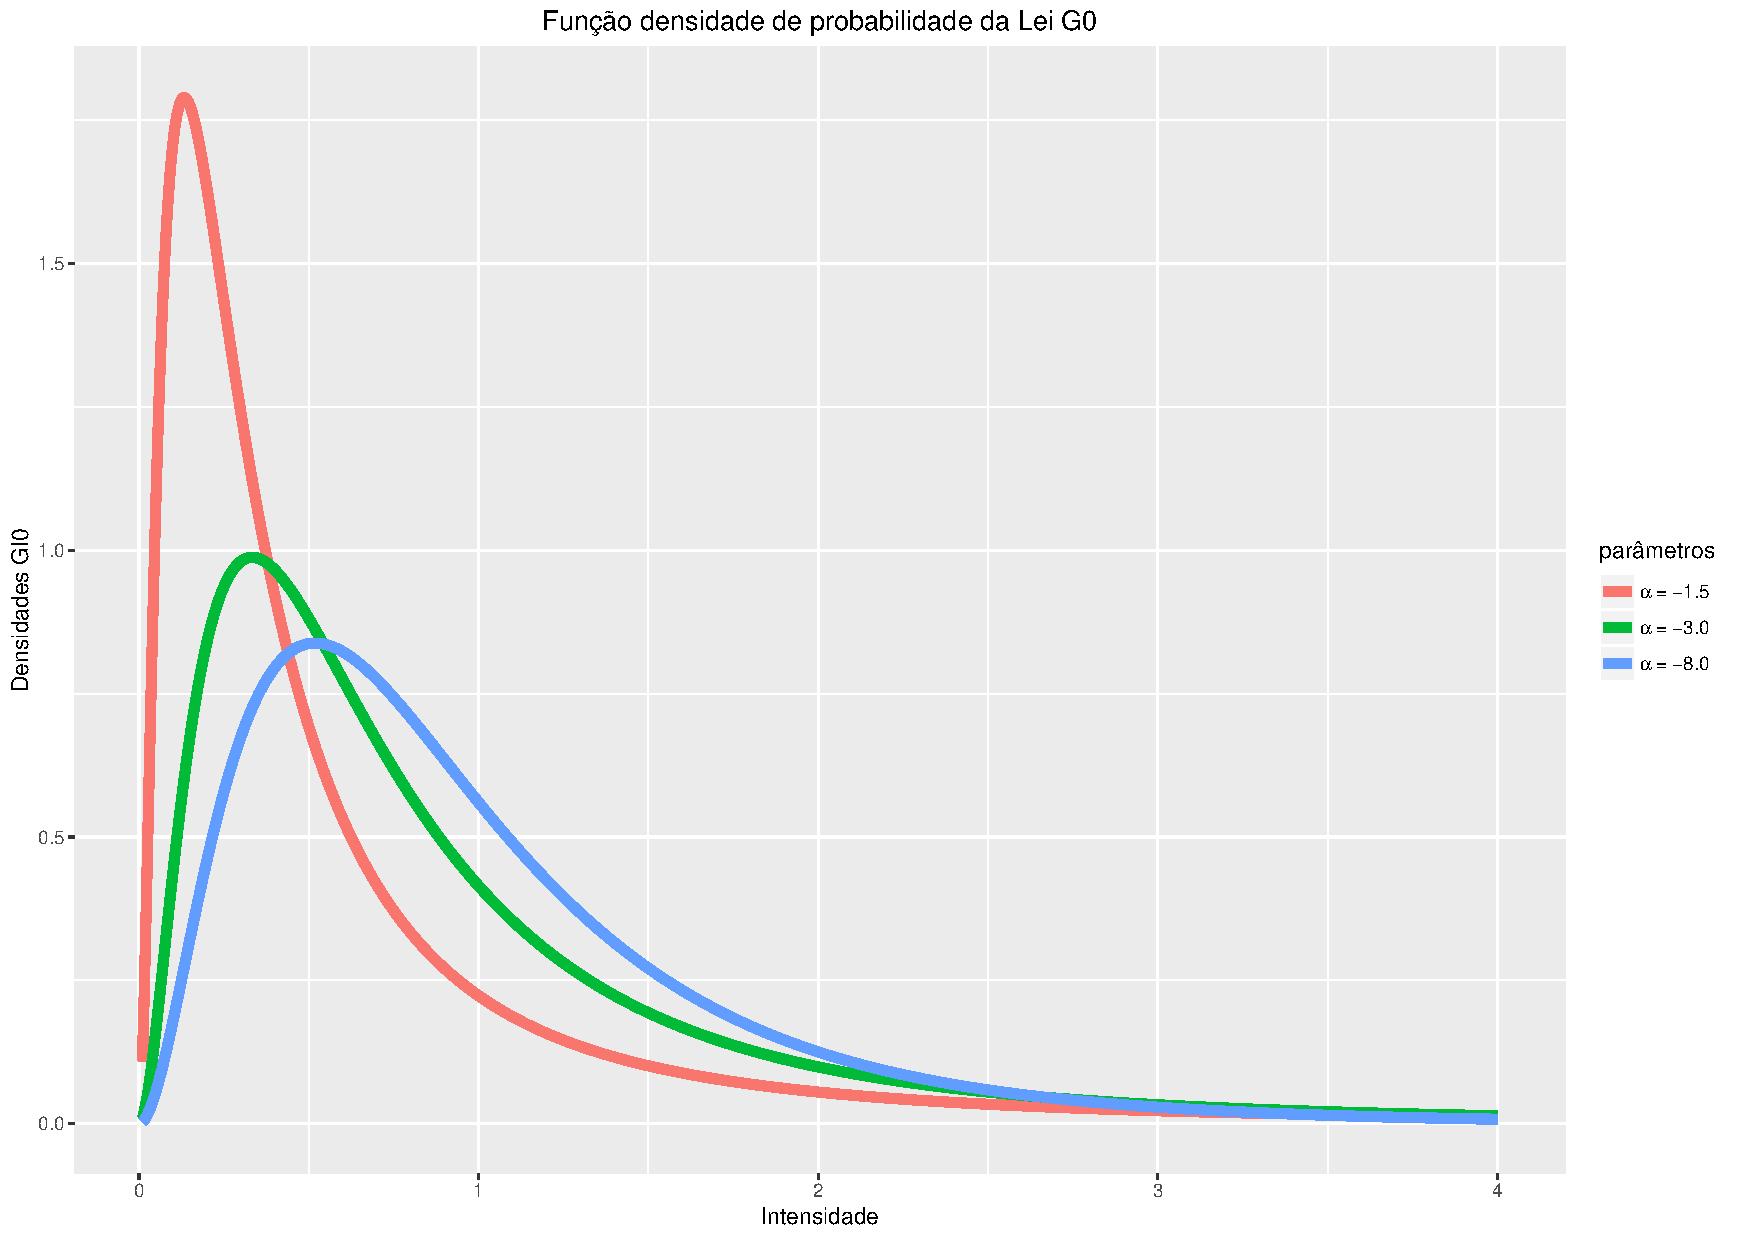
\includegraphics[scale=0.5]{plots/GI0Densities.pdf}
     \caption{Densidades da distribuição $G_I^0(\alpha, -\alpha - 1, 3)$, com $\alpha \in \left \{  -8.0, -3.0, -1.5 \right \}$}
     \label{graf_1}
\end{figure}
%%% ACF Os gráficos devem estar em português.
%%% ACF A cada gráfico associe o arquivo e linha que o produz, como um comentário.
%%% ACF Ilustre também as densidades em escala semilogarítmica, acrescente a densidade gama de parâmetro de forma 3 (o caso limite para $\alpha\to-\infty$) 
%%% ACF Faça outro gráfico mostrando a variação com o número de looks, mantendo a média constante

Já na figura abaixo temos o resultado do histograma feito a partir de um conjunto de $10.000$ variáveis aleatórias $G_I^0$ geradas a partir da função que segue o Modelo Multiplicativo, conforme explicado anteriormente. Juntamente a esse histograma, temos o traçado da curva de densidade de probabilidade e, com isso, é possível perceber um determinado ajuste entre ambos.

% GI0 Generation
\begin{figure}[H]
     \centering
     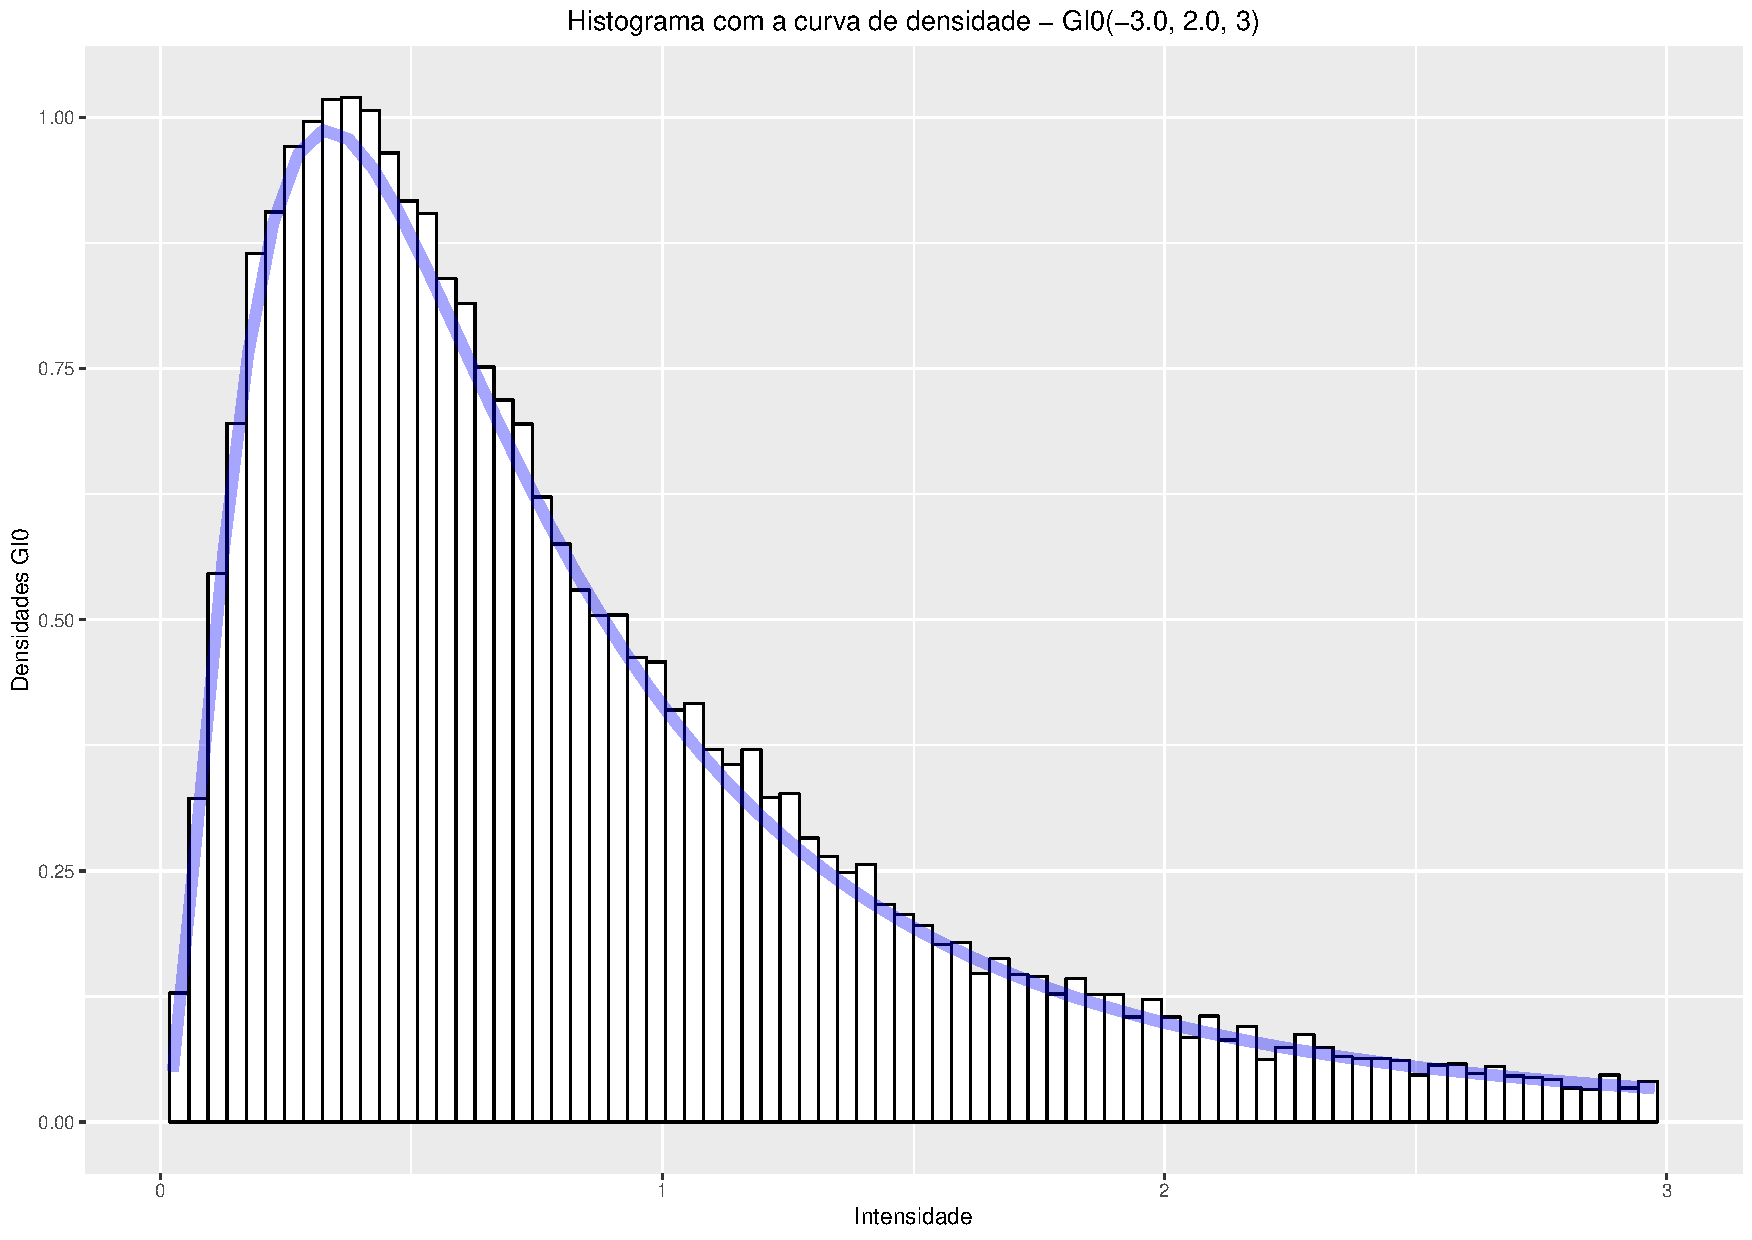
\includegraphics[scale=0.5]{plots/GI0RandVar.pdf}
     \caption{Histograma de variáveis aleatórias $G_I^0(-3.0, 2.0, 3)$ juntamente com sua densidade de probabilidade}
     \label{graf_2}
\end{figure}
%%% ACF A densidade não está suave o suficiente. Use mais pontos.

Vale reforçar que sistemas que empregam iluminação coerente são usados para explorar regiões inacessíveis e/ou inobserváveis (a superfície de Vênus, o interior do corpo humano, o fundo do mar, áreas sob nebulosidade, etc.). É, portanto, de suma importância poder fazer inferências confiáveis sobre o tipo de alvo em análise, uma vez que informações visuais raramente estão disponíveis.

				
%=========================================================

\section{Introdução à Estatística Inferencial}

Conforme \citet{CasellaBergerStatisticalInference}, uma variável aleatória é caracterizada ou descrita pela sua distribuição de probabilidade. Esta, por sua vez, é descrita pelos seus parâmetros populacionais. Existe um grande interesse em conhecer os parâmetros populacionais da distribuição que se está trabalhando para conhecer como os dados estão se comportando. Como geralmente tais parâmetros não são conhecidos, é preciso desenvolver procedimentos para estimá-los. Desse modo, as estimativas dos parâmetros populacionais são obtidas a partir de variáveis aleatórias de uma amostra representativa da população.
 
As estimativas dos parâmetros populacionais da distribuição são realizadas a partir dos resultados (dados) de uma variável aleatória de uma amostra representativa extraída da população em questão. A esse procedimento damos o nome de estatística inferencial, visto que se está inferindo algo da população a partir de uma amostra populacional.

Existem basicamente duas formas de estimação de parâmetros: por ponto (pontual) ou por intervalo de confiança. De forma breve, a estimativa pontual é um valor obtido a partir dos resultados (dados) de uma variável aleatória de uma amostra representativa da população. 
Por outro lado, a estimação de parâmetros por intervalo de confiança consiste em gerar um intervalo que inclui a estimativa pontual, no qual se admite que esteja o parâmetro da população.
As formas são complementares, sendo que a segunda está associada ao conceito de teste de hipóteses. 

As técnicas usuais de inferência incluem métodos baseados no princípio de analogia, sendo os estimadores estatísticos de ordem e momento os mais populares desta classe, e no princípio de Máxima Verossimilhança. Entretanto, além dessas técnicas existem os estimadores baseados em Log-Cumulantes ou também chamados de Log-Momentos e os baseados na Teoria da Informação, mais precisamente em Distâncias Estocásticas. Esses dois últimos possuem propriedades bem interessantes e têm sido alvos de pesquisa em diversos trabalhos encontrados na literatura. Neste trabalho, foram estudados e implementados ao todo quatro algoritmos de estimação: Método da Máxima Verossimilhança, Método dos Momentos, Método dos Log-Cumulantes (Log-Momentos) e Método de Distâncias Estocásticas. Nas seções seguintes estão descritas informações a respeito dessas quatro técnicas.

\section{Estimação por Máxima Verossimilhança (MV)}

\subsection{Introdução}

A ideia básica deste método é bem intuitiva. Parece razoável que uma boa estimativa do parâmetro desconhecido \begin{math} \theta \end{math} seria o valor que maximiza a credibilidade de se obter os dados que são observados. 
É por conta dessa ideia que esse método de estimação é denominado de Máxima Verossimilhança. 
 
Conforme descrito no livro de \citet{CasellaBergerStatisticalInference}, suponha que tenhamos uma amostra aleatória \begin{math} \bm X = (X_{1}, X_{2}, \dots, X_{n}) \end{math} para a qual a função de densidade de probabilidade de cada \begin{math} X_{i} \end{math} é \begin{math} f(x_{i}; \theta)\end{math}, e que as variáveis aleatórias sejam independentes.

Então, a função de densidade de probabilidade conjunta da amostra aleatória \begin{math} X \end{math}, denotada por \begin{math} L(\theta) \end{math} é dada por:
%%% ACF Aqui temos um conflito de notação: $L$ foi definido como o número de loooks. Sugiro usar $\mathcal L$ para a verossimilhança
\begin{equation}
L(\theta) = P (X_{1} = x_{1}, \dots, X_{n} = x_{n}) =  f(x_{1}; \theta) \cdots f(x_{n}; \theta) =  \prod_{1}^{n} f(x_{i}; \theta).
\end{equation}

A segunda igualdade escrita acima é proveniente do fato de que temos uma amostra aleatória, o que implica, por definição, que cada \begin{math} X_{i} \end{math} seja independente e igualmente distribuída. Agora, à luz da ideia básica da estimação por máxima verossimilhança, uma maneira razoável de proceder é tratar a função de verossimilhança dada por \begin{math} L (\theta) \end{math} como uma função de \begin{math} \theta \end{math}, e encontrar o valor do parâmetro que a maximiza.

No contexto das imagens SAR, os estimadores de Máxima Verossimilhança são amplamente utilizados, uma vez que possuem boas propriedades ótimas bem conhecidas, como consistência, eficiência e normalidade assintótica, entre outras. 
Por exemplo, esses estimadores foram utilizados para a análise de imagens SAR sob o modelo $K$ no trabalho de \citet{KMaxVer_Joughin}.

\subsection{Estimadores MV para os parâmetros da lei $G_I^0$}

Então como visto, dado uma amostra $\bm Z = (Z_1, Z_2, \dots, Z_N)$ e supondo que essas observações são resultados de variáveis aleatórias independentes e identicamente distribuídas que seguem a distribuição $D(\theta)$, com $\theta \in \Theta$, um estimador de Máxima Verossimilhança para $\theta$ é dado por
\begin{equation}
    \widehat{\theta} = \arg\max L(\theta; z) \text{, para } \theta \in \Theta, \label{eq:mv}
\end{equation}
em que $L$ é a função de verossimilhança da amostra $Z$ sob o parâmetro $\theta$. Podemos utilizar as propriedades logarítmicas para simplificar os cálculos, aplicando o logaritmo natural, visto que se trata de uma função positiva e que o ponto que produz o máximo da função não varia, independentemente de aplicar ou não o logaritmo. 
Além disso, sob várias condições é equivalente e muitas vezes mais fácil trabalhar com a função log-verossimilhança reduzida $ \ell (\theta; Z)$, onde todos os termos que não dependem de $\theta$ são ignorados.

Embora a maximização direta de~\eqref{eq:mv} seja possível (seja analiticamente ou usando ferramentas numéricas) e desejável, muitas vezes encontramos estimadores de MV resolvendo o sistema de equações (geralmente não-lineares) dado por
\begin{equation}
    \nabla \ell (\widehat{\theta}) = \bm 0, \label{eq:gradient} 
\end{equation}
em que $\nabla$ denota o gradiente. 
Segundo \citet{FreryMinute2004}, a escolha entre resolver~\eqref{eq:mv} ou~\eqref{eq:gradient} depende muito de questões computacionais: disponibilidade de algoritmos confiáveis, esforço computacional necessário para implementar e/ou obter a solução e assim por diante. 
Essas equações, em geral, não têm solução explícita.

Para a construção dos estimadores de Máxima Verossimilhança para o modelo $G_I^0$, considere $\bm Z = (Z_1, Z_2, \dots, Z_N)$ uma amostra aleatória de $N$ variáveis, independentes e igualmente distribuídas, que seguem essa distribuição. 
Os parâmetros $\alpha$ e $\gamma$ são desconhecidos, enquanto que o parâmetro \textit{Looks} ($L$) é conhecido. 
Nesse caso, a função de verossimilhança é $L((\alpha, \gamma); Z) = \prod_{i=1}^{N} f_Z(Z_i)$, em que $f_Z$ é a função densidade de probabilidade definida anteriormente em \eqref{eq:fdpGI0}. 

Assim, a função de log-verossimilhança ($\log L$) é escrita como
\begin{equation}
    \log L((\alpha, \gamma); Z) = N\log \frac{L^{L}\Gamma(L-\alpha)}{\gamma^{\alpha}\Gamma(-\alpha)\Gamma(L)} +  (L-1)\sum_{i=1}^{N}\log Z_i - (L-\alpha)\sum_{i=1}^{N}\log (\gamma + Z_iL). \label{eq:logVer}
\end{equation}

A partir da função acima, podemos escrever a função de log-verossimilhança reduzida, excluindo os termos que não dependem de $\alpha$ e $\gamma$:
\begin{equation}
    \ell ((\alpha, \gamma); Z) = N\log\Gamma(L-\alpha) - N\alpha \log\gamma - N\log\Gamma(-\alpha) - (L-\alpha)\sum_{i=1}^{N}\log(\gamma +Z_iL). \label{eq:logVerRed}
\end{equation}

O sistema de equações representado em \eqref{eq:gradient} é, em nosso caso, dado por
\begin{align}
  \frac{\partial l}{\partial \widehat{\alpha}} &= N[\Psi(-\widehat{\alpha}) - \Psi(L-\widehat{\alpha})] + \sum_{i=1}^{N}\log\frac{\widehat{\gamma} + Z_iL}{\widehat{\gamma}} = 0,\\
   \frac{\partial l}{\partial \widehat{\gamma}} &= -N\frac{\widehat{\alpha}}{\widehat{\gamma}} - (L - \widehat{\alpha})\sum_{i=1}^{N}(\widehat{\gamma} + Z_iL)^{-1} = 0,
\end{align}
em que $\Psi(\tau) = \frac{\textit{d}log\Gamma(\tau)}{\textit{d}\tau}$ é a função \textit{Digama}. Resolvendo esse sistema de equações obtemos os estimadores para os parâmetros $\alpha$ e $\gamma$ da distribuição $G_I^0$, denotados por $\widehat{\alpha}$ e $\widehat{\gamma}$. Em geral, nenhuma solução explícita para este sistema está disponível e, portanto, rotinas numéricas têm que ser usadas.

Assumindo a simplificação feita para o parâmetro de escala ($\gamma^{*} = -\alpha - 1$), temos que o estimador de Máxima Verossimilhança para o parâmetro $\alpha$, denotado por $\widehat{\alpha}$, é dado pela solução da seguinte equação não linear:
\begin{align}
    \Psi(-\widehat{\alpha}) - \Psi(L-\widehat{\alpha}) - \log(-\widehat{\alpha}-1) - \frac{\widehat{\alpha}}{\widehat{\alpha}+1} + \nonumber \\ 
    \frac{1}{N}\sum_{i=1}^{N}\log(-\widehat{\alpha} - 1 + LZ_i) - \left ( \frac{\widehat{\alpha}-L}{N} \right )\sum_{i=1}^{N}(-\widehat{\alpha} - 1 + LZ_i)^{-1} = 0.
\end{align}

% MOMENTOS 
\section{Estimação pelo Método dos Momentos (MM)}

\subsection{Introdução}

Uma outra forma de encontrar estimadores de parâmetros populacionais, como a média e a variância por exemplo, é através do método dos momentos. Este método é baseado na comparação dos momentos teóricos com os momentos amostrais das variáveis aleatórias envolvidas, a partir de uma amostra de $N$ observações. 

Em suma, o método dos momentos envolve equacionar momentos da amostra com momentos teóricos. Então, vamos começar lembrando as definições dos momentos teóricos, bem como aprender as definições dos momentos das amostras.

A seguir estão algumas definições:
\begin{enumerate}
	\item $E(X^k)$ é o k-ésimo momento teórico da distribuição 
    \item $M_k=\dfrac{1}{N}\sum\limits_{i=1}^N X_i^k$ é o k-ésimo momento amostral 
\end{enumerate}

A ideia por trás desse método é bastante simples. Vejamos os seguintes passos da primeira forma de se calcular os estimadores por este método, utilizando o primeiro e o segundo momento:
\begin{enumerate}
  \item Equacione o primeiro momento da amostra  $M_1=\dfrac{1}{N}\sum\limits_{i=1}^N X_i=\bar{X}$ ao primeiro momento teórico $E(x)$
  \item Equacione o segundo momento da amostra $M_2=\dfrac{1}{N}\sum\limits_{i=1}^N X_i^2$ ao segundo momento teórico $E(x^2)$
  \item Continuar igualando momentos amostrais, $M_k$, com os correspondentes momentos teóricos  $E(X^k)$, $k = 3, 4, \dots $, até que se tenha tantas equações quanto se tem de parâmetros.
  \item Por fim, basta resolver o sistema e calcular os estimadores para os parâmetros.
\end{enumerate}

Os valores resultantes são chamados de estimadores de método de momentos. Parece razoável que esse método forneça boas estimativas, já que a distribuição empírica converge, em certo sentido\footnote{A convergência é no sentido da Lei dos Grandes Números, isto é, convergência em probabilidade}, para a distribuição de probabilidade. Portanto, os momentos correspondentes devem ser aproximadamente iguais. Desse modo, estimadores de momentos são favorecidos em aplicações, já que são fáceis de derivar e são, em geral, computacionalmente atraentes. De certo modo, são mais simples de calcular em relação ao método de Máxima Verossimilhança, entretanto podem gerar, com mais frequência, estimadores menos precisos. 

Então, de modo resumido, seja $Z$ uma variável aleatória contínua com função densidade de probabilidade $f_Z(z)$, os momentos teóricos são dados por $m_j = \int x^jf_Z(z)dz$. Os momentos amostrais, por sua vez, são definidos como $\widehat{m_j} = N^{-1}\sum_{i=1}^{N}z_i^j$. Após calcular os momentos teóricos e amostrais, o processo de inferência é simples e consiste em comparar os momentos amostrais, $\widehat{m_j}$, com os correspondentes momentos teóricos, $m_j$, até se ter tantas equações quantos forem os parâmetros a serem estimados. De posse do sistema de equações, basta resolver e calcular os estimadores para os parâmetros. Essa é a ideia geral de funcionamento do Método dos Momentos implementado neste trabalho.

\subsection{Estimadores de Momentos para os parâmetros da $G_I^0$}

Para estimar os parâmetros $\alpha$ e $\gamma$ da distribuição $G_I^0(\alpha, \gamma, L)$, é necessário estimar dois momentos. 
Neste relatório, serão utilizados momentos de ordem $\frac{1}{2}$ e $1$, ou seja, $m_{1/2}$ e $m_1$ respectivamente. 
Esses momentos, de acordo com a equação \eqref{eq:moments}, são dados por
%%% ACF Mudou a notação de M para m?
\begin{align}
    m_{1/2} &= \left ( \frac{\gamma}{L}\right )^{1/2} \frac{\Gamma(-\alpha-1/2)\Gamma(L+1/2)}{\Gamma(-\alpha)\Gamma(L)}  \text{ para } \alpha < -1/2 \label{eq:m12}, \text{ e }\\
    m_{1} &= \left ( \frac{\gamma}{L}\right ) \frac{\Gamma(-\alpha-1)\Gamma(L+1)}{\Gamma(-\alpha)\Gamma(L)} \text{ para } \alpha < -1. \label{eq:m1}
\end{align}

Podemos utilizar o momento $\widehat{m}_{1/2}^2$ para auxiliar nos cálculos e utilizar as equações acima \eqref{eq:m12} e \eqref{eq:m1} para determinar o estimador $\widehat{\alpha}$ que pode ser dado como solução da seguinte equação
\begin{equation}
    g(\widehat{\alpha}) - \zeta = 0,
\end{equation}
em que 
\begin{equation}
    g(\widehat{\alpha}) = \frac{\Gamma^2(-\widehat{\alpha} - 1/2)}{\Gamma(-\widehat{\alpha})\Gamma(-\widehat{\alpha} - 1)}
\end{equation}
e
\begin{equation}
    \zeta = \frac{\widehat{m}_{1/2}^2\Gamma(L)\Gamma(L+1)}{\widehat{m}_{1}\Gamma^2(L+1/2)}.
\end{equation}
Dessa forma, encontrando o valor de $\widehat{\alpha}$ e o substituindo na equação \eqref{eq:m12} ou na equação \eqref{eq:m1}, obtemos o estimador $\widehat{\gamma}$.

Como já mencionado, podemos simplificar o processo de estimação do parâmetro $\gamma$, obtendo-o este de tal forma que o valor esperado $E(Z^r)$ tenha valor unitário e, assim, definimos ele em função do parâmetro $\alpha$. Como já citado antes o valor de $\gamma^{*}$ vale $-\alpha - 1$. Contudo, abaixo está o cálculo a partir de \eqref{eq:moments} que levou a essa conclusão:
\begin{equation}
    E(Z^r) = 1 \Rightarrow \left (\frac{\gamma*}{L}\right ) \frac{\Gamma(-\alpha-1)\Gamma(L+1)}{\Gamma(-\alpha)\Gamma(L)} = 1 \Rightarrow \gamma* = L\left ( \frac{\Gamma(-\alpha)\Gamma(L)}{\Gamma(-\alpha-1)\Gamma(L+1)} \right ) ,
\end{equation}
e, sabendo que $\Gamma(n) = (n-1)!$, temos que
\begin{equation}
    \gamma^{*} = -\alpha - 1.
\end{equation}

Estimadores de momentos fracionários foram utilizadas amplamente em \citet{Clutter1997}. Dessa forma, assumindo a simplificação acima e utilizando $r=\frac{1}{2}$ na equação do $r$-ésimo momento da $G_I^0$ dada em \eqref{eq:moments} é preciso resolver a equação a seguir para se obter o estimador de momentos denotado por $\widehat{\alpha}$.
\begin{equation}
    \frac{1}{N}\sum_{i=1}^{N}\sqrt{z_i}-\sqrt{\frac{-\widehat{\alpha} - 1}{L}}\frac{\Gamma(-\widehat{\alpha} - \frac{1}{2})}{\Gamma(-\widehat{\alpha})}\frac{\Gamma(L+\frac{1}{2})}{\Gamma(L)} = 0 .\label{fractional_moments}
\end{equation} 

% LOG-CUMULANTES
\section{Estimação pelo Método dos Log-Cumulantes (MLC)}

\subsection{Introdução}

Sabe-se que a estimação de parâmetros de funções de densidade de probabilidade é um dos principais passos na área de processamento de imagens e sinais estatísticos. Nesse contexto, o método de log-cumulantes (MLC) consiste em um método de estimação de parâmetros proposto por \citet{nicolas2002} e tem sido utilizado com resultados satisfatórios em processamentos de imagens SAR.

O Método de Log-cumulantes pode ser visto como uma alternativa às abordagens clássicas de máxima verossimilhança (MV) e método dos momentos (MM). 
Estudos feitos no trabalho de \citet{krylov2013} derivaram uma condição geral suficiente para a consistência forte das estimativas de MLC, que representa uma importante propriedade assintótica de qualquer estimador estatístico. 
Este resultado permite a demonstração da consistência forte das estimativas de MLC para uma seleção de famílias de distribuição amplamente utilizadas originárias de processamento de imagem de radar de abertura sintética, contudo não é restrito somente a esse campo. 

Nesse sentido, estimadores baseados em log-cumulantes têm ganhado espaço na literatura devido às suas boas propriedades e bom desempenho. 
No contexto de processamento de imagens SAR, este método é especialmente utilizado quando se tem pequenas amostras que se trata de um problema crítico em várias aplicações. 
Ainda no trabalho de \citet{krylov2013}, foram destacados que os resultados obtidos sugerem que o MLC é uma alternativa viável e computacionalmente rápida que é especialmente útil quando a abordagem direta do estimador de Máxima Verossimilhança se mostra inviável. 

Pesquisadores têm utilizado os parâmetros estimados pelo método de log-cumulantes como entradas, por exemplo, para métodos de classificação de imagens SAR e detecção de mudanças em imagens SAR multitemporais. 
A seguir é apresentado o MLC conforme proposto e analisado no trabalho de \citet{nicolas2002}.

\subsection{Definição}

Seja $Z$ uma variável aleatória contínua com função densidade de probabilidade $f_Z(z, \theta)$ definida em $\mathbbm{R}^{+}$. O Método de log-cumulantes, baseado na transformada de Mellin de $f_Z(z, \theta)$, é definido como:
\begin{equation}
    \phi_{Z}(s) = \int_{0}^{\infty} u^{s-1} f_{Z}(u, \theta)du = E(Z^{s-1}) \label{eq:logcum}
\end{equation}
com $s$ sendo um número complexo com norma unitária \citep{nicolas2002}.

Existem dois conceitos importantes para a construção de estimadores utilizando o método de log-cumulantes que são os log-momentos e log-cumulantes de ordem $v$. É possível obter expressões analíticas para os log-momentos e log-cumulantes de ordem $v$ por simples derivações de $\phi_{Z}(s)$, avaliadas em $s = 1$. O log-momento de ordem $v$ pode ser definido como:
\begin{equation}
    \widetilde{m}_{v} = {\left.
    \frac{d^{v}\phi_{Z}(s)}{ds^{v}} 
    \right\vert}_{s=1} ,  v \in \mathbbm{N}
    \label{eq:logmomV}
\end{equation}
%%% ACF Não consegui fazer com que a barra vertical fique do tamanho da fração :-(

Tomando como base o logaritmo natural ($\ln$) de $\phi_{Z}(s)$, pode-se obter o log-cumulante de ordem $v$ de forma bem similar e análoga à equação anterior. Temos que:
\begin{equation}
    \widetilde{k}_{v} = \frac{d^{v}\psi_Z(s)}{ds^{v}}\Bigr|_{\substack{s=1}} ,  v \in \mathbbm{N},
    \label{eq:logcumV}
\end{equation}
com $\psi_Z(s) = \log(\phi_{Z}(s))$.

O funcionamento e estratégia do método de log-cumulantes para estimar o vetor de parâmetros desejado $\theta$ se baseia na relação entre os log-momentos e log-cumulantes que é dada pela seguinte equação:
\begin{equation}
    \widetilde{k}_{v} = \widetilde{m}_{v} - \sum_{i=1}^{v-1}\binom{v-1}{i-1}\widetilde{k}_{i}\widetilde{m}_{v-i},
\end{equation}
%%% ACF Defina os novos elementos desta equação

Desta equação acima, pode-se destacar como exemplo os log-momentos e log-cumulantes de ordem $1$, $2$ e $3$ que, por sua vez, obedecem a seguinte relação:
%%% ACF Use a pontuação adequada
\begin{equation}
    \begin{matrix}
        \widetilde{k}_{1} = \widetilde{m}_{1} \\ 
        \widetilde{k}_{2} = \widetilde{m}_{2} - \widetilde{m}_{1}^{2} \\
        \widetilde{k}_{3} = \widetilde{m}_{3} - 3\widetilde{m}_{1}\widetilde{m}_{2} + 2\widetilde{m}_{1}^{3} 
    \end{matrix}  
    \label{eq:logcum123}
\end{equation}

Na maioria das vezes, $\widetilde{k}_{v}$ é calculado como função do vetor de parâmetros $\theta$ e o processo de estimação de $\theta$ é feito substituindo $\widetilde{m}_{v}$ pelo correspondente log-momento amostral, que é dado por:
\begin{equation}
    \widehat{\widetilde{m}}_{v} = \frac{1}{n}\sum_{i=1}^{n}\log z_{i}^{v},
    \label{eq:log_momAmostrais}
\end{equation}
em que $z_i$, $i \in \{1, 2, \dots, n\}$, é uma amostra da variável aleatória $Z$ que segue uma determinada distribuição de probabilidade. A seguir serão mostradas as etapas de construção dos estimadores dos parâmetros da $G_I^0$ mediante utilização do método de log-cumulantes (MLC). 

\subsection{Estimadores MLC para os parâmetros da $G_I^0$}

Para a distribuição $G_I^0$, a função $\phi_{Z}(s)$ é obtida por meio da equação dada anteriormente em~\eqref{eq:logcum}, isto é, precisamos utilizar a equação do $r$-ésimo momento da $G_I^0$ dada em \eqref{eq:moments} para obter a expressão para $E(Z^{s-1})$. Portanto, temos:
%%% ACF Não exagere com os \quad; veja como eu fiz acima
\begin{equation}
    \phi_{G_I^0}(s) = \left ( \frac{\gamma}{L} \right )^{s-1}\frac{\Gamma(1-s-\alpha)\Gamma(L+s-1)}{\Gamma(-\alpha)\Gamma(L)}  \qquad \alpha \quad \text{<} \quad -s+1
\end{equation}

Utilizando a expressão acima obtida para $\phi_{G_I^0}(s)$ na equação dada em \eqref{eq:logcumV}, obtém-se o seguinte sistema de equações:
%%% ACF Por que matrix? Use alinhamento como eu fiz acima
\begin{equation}
    \begin{matrix}
        \widetilde{k}_{1} = \log \left ( \frac{\gamma}{L} \right ) + \Psi^{0}(L) - \Psi^{0}(-\alpha)  \\ 
        \widetilde{k}_{2} = \Psi^{1}(L) - \Psi^{1}(-\alpha)
    \end{matrix}
\end{equation}
em que $\Psi^{0}(.)$ e $\Psi^{1}(.)$ correspondem às funções \textit{digama} e \textit{trigama}, respectivamente.

%%% ACF Precisa usar o transposto? Se sim, defina.
Portanto, para estimar o vetor de parâmetros dado por $\theta = (\alpha, \gamma)^{\top}$ da distribuição $G_I^0$, basta aplicarmos as duas primeiras equações do sistema dado em \eqref{eq:logcum123} que representam os valores de $\widetilde{k}_{1}$ e $\widetilde{k}_{2}$ e as equações encontradas logo acima. Por fim, para estimar os parâmetros, basta substituir os valores de $\widetilde{m}_{1}$ e $\widetilde{m}_{2}$ pelos correspondentes log-momentos amostrais dados pela equação \eqref{eq:log_momAmostrais}. 

Assumindo a simplificação feita de que $\gamma^{*} = -\alpha - 1$, o estimador Log-cumulante do parâmetro $\alpha$ da $G_I^0$ é dado pela solução de $\widehat{\widetilde{k}_{1}} = \log \frac{1-\widehat{\alpha}}{L} + \Psi^{0}(L) - \Psi^{0}(-\alpha)$. Como sabemos que $\widehat{\widetilde{k}}_{1} = \widehat{\widetilde{m}}_{1} = n^{-1}\sum_{i=1}^{n}\log z_i$, então para encontrar o estimador $\widehat{\alpha}$ pelo MLC basta encontrar a solução para:
\begin{equation}
    \frac{1}{n}\sum_{i=1}^{n}\log z_i - \log \left ( \frac{-\widehat{\alpha}-1}{L} \right ) - \Psi^{0}(L) + \Psi^{0}(-\alpha) = 0
    \label{eq:alphaEst_logCum}
\end{equation}

\section{Estimação baseada em Distâncias Estocásticas}

\subsection{Introdução}

Nos últimos anos, houve um crescente interesse em adaptar ferramentas de Teoria da Informação para processamento de imagens. 
Em particular, o processamento de imagens polarimétricas também obteve benefícios com esse conceito, uma vez que medidas de divergência podem ser adotadas para fornecer métodos de avaliar algoritmos de segmentação. 
Ademais, no trabalho de \citet{Goudail:04} a distância de Bhattacharyya foi proposta como um meio de fornecer uma medida de contraste escalar para imagens de SAR polarimétrica e interferométrica.

Nesse contexto, temos que a teoria da informação tem sido amplamente aplicada à estatística e teoria da probabilidade, obtendo determinado sucesso. 
\citet{Shannon48} propôs em seu artigo a informação $I(X,Y)$ entre as variáveis aleatórias $X$ e $Y$ como sendo uma divergência calculada usando as funções de densidade correspondentes $P_{X}$ e $P_{Y}$.
%%% ACF Você vinha utilizando f para denotar densidades; por que mudou?
Essas divergências foram amplamente estudadas por Kullback e Leibler, e Renyi, entre outros autores. 
Essas divergências têm múltiplas aplicações no processamento de sinais e imagens \citep{Aviyente}, classificação de texturas e detecção automática de regiões em imagens SAR.

\subsection{Divergências e Distâncias Estocásticas}

Conforme \citet{tese_abraao}, existem diversos parâmetros de separabilidade, que também são comumente chamados de medidas de distância entre distribuições, que possuem o objetivo de determinar o quão similares são duas distribuições de probabilidade. 
Nesse contexto, surge o conceito da divergência que se configura justamente como uma medida de distância e cuja definição surgiu com o desenvolvimento da Teoria da Informação. 

De maneira formal, a divergência pode ser definida como uma função não negativa entre duas medidas de probabilidade que obedece as propriedades de definitividade e não negatividade. 
Se a função também é simétrica, ela é chamada de ``distância''. 
Nesse sentido, se a distância também satisfaz a desigualdade triangular, ela é conhecida como ``métrica''. 
Por meio do conceito de divergência é que se obtém distâncias entre distribuições de probabilidade. 
Essas propriedades citadas anteriormente relativas à divergência --definitividade, não negatividade e simetria-- são melhor explicadas posteriormente.

Uma imagem pode ser vista como um conjunto de regiões, em que cada uma possui seus pixels descritos por uma variável aleatória que, por sua vez, segue uma determinada distribuição. 
Assim, \citet{Nascimento2010} propuseram medidas de contraste baseadas em divergências estocásticas para quantificar diferenças entre áreas de imagens SAR. 

Segundo \citet{tese_abraao}, após os primeiros conceitos de divergência, deu-se início ao estudo de classes desta medida. 
Entre elas pode-se citar a classe de divergências $\phi$ ou família de divergências $\phi$ desenvolvida no trabalho de \citet{Csiszar67}. 
Esta classe é caracterizada por um procedimento analítico sistematizado e formalizado que permite se obter medidas de divergência a partir da escolha apropriada de uma função convexa $\phi$. 
Esse estudo foi posteriormente estendido por \citet{salicruetal1993}, no qual foi inserida nesse contexto a função $h$ que permitiu a geração de expressões para uma quantidade maior de divergências conhecidas em relação ao trabalho anterior feito por Csiszár. 
%%% ACF Atente para a notação correta da família h-\pni, para que não pareça uma subtração
A nova família de divergências ficou conhecida como família $h$-$\phi$. 

Sabemos que, por meio de medidas de divergência, é possível se obter expressões para distâncias entre distribuições de probabilidade que, por sua vez, recebem a denominação de distâncias estocásticas ou simplesmente distâncias. 
De modo geral, uma distância estocástica é uma divergência que além de satisfazer as propriedades de não-negatividade e definitividade, satisfaz a propriedade de simetria. 
Conforme estudo feito no livro de \citet{StatisticalInferenceBasedonDivergenceMeasures}, a definição formal de distância estocástica será dada a seguir. 
\begin{quote}
    \textbf{Definição de distância estocástica:} Uma distância estocástica definida em um conjunto (domínio) $\nu$ é uma função $ d_\phi^h\colon \nu \times \nu \rightarrow \mathbbm{R} $, em que o contradomínio $\mathbb{R}$ é o conjunto dos números reais, que trata de associar cada par ordenado de elementos $X, Y \in \nu$, que representam variáveis aleatórias, a um número real denotado por $d_\phi^h(X, Y)$. Esta associação é feita de modo que sejam satisfeitas três importantes condições/propriedades para todo e qualquer $X, Y \in \nu$. Tais condições já discutidas anteriormente são descritas a seguir.
    \begin{enumerate}
        \item \textit{Definitividade}: $d_\phi^h(X, Y) = 0 \Leftrightarrow X = Y$;
        \item \textit{Não-Negatividade}: Se $X \neq Y$, então temos $d_\phi^h(X, Y)$ \text{>} $0$;
        \item \textit{Simetria}: $d_\phi^h(X, Y) = d_\phi^h(Y, X)$
    \end{enumerate}
\end{quote}

Um caso particular ocorre quando temos $X$ e $Y$ pertecendo a mesma distribuição de probabilidade, porém com parâmetros diferentes. Nessa situação, é suficiente escrever a notação $d_\phi^h(\theta_1, \theta_2)$. Desse modo, temos que $d_\phi^h(\theta_1, \theta_2) \geq 0$ em que $d_\phi^h(\theta_1, \theta_2) = 0$ se, e somente se $\theta_1 = \theta_2$. Tendo essa igualdade de parâmetros, consequentemente as variáveis $X$ e $Y$ possuem a mesma distribuição e a distância entre elas é nula. Em suma, distâncias estocásticas são utilizadas para comparar e analisar distribuições de probabilidade definidas no mesmo espaço de probabilidades.

\subsection{Introdução à Inferência por distâncias para a lei $G_I^0$}

No contexto da estimação de parâmetros, estamos interessados em distâncias entre funções de densidade de probabilidade. 
Neste trabalho, foi utilizado esse conceito de distância da Teoria da Informação para encontrar o melhor valor para o parâmetro de rugosidade ou textura da distribuição $G_I^0$ --o parâmetro $\alpha$-- de modo que a distribuição empírica de dados seja aproximada pela função de densidade de probabilidade da $G_I^0$. 
Em outras palavras, a ideia principal consiste de, dada a amostra de dados $\bm z$, calcular $\widehat{\alpha}$, estimador de $\alpha$, como sendo o ponto do espaço paramétrico que minimiza a distância entre a função densidade $f_{G_I^0}$ e uma estimativa da função de densidade subjacente que caracteriza o modelo, isto é, a distribuição empírica dos dados da amostra. 
O custo computacional de avaliar cada ponto é relativamente pequeno, visto que o histograma está fixado e a densidade não envolve funções especiais. 

Nesse contexto, é possível encontrar o mínimo da distância em função do parâmetro $\alpha$ da lei $G_I^0$, o qual provê uma forma de estimação do parâmetro. 
Sejam $V$ e $W$ duas variáveis aleatórias definidas sobre o mesmo espaço de probabilidades cujas funções densidade são dadas por $f_V(x; \theta_1)$ e $f_W(x; \theta_2)$. 
Assim, podemos definir como exemplo as seguintes distâncias estocásticas que são bastante discutidas na literatura:
\begin{enumerate}
    \item \textbf{Distância de Hellinger}: $$ d_H(V,W) = 1 - \int_{-\infty}^{\infty}\sqrt{f_V f_W}.$$
    \item \textbf{Distância de Bwidehattacharyya}: $$d_B(V,W) = -\log\int_{-\infty}^{\infty}\sqrt{f_V f_W}.$$
    \item\textbf{Distância Triangular}: $$d_T(V,W) = \int_{-\infty}^{\infty}\dfrac{(f_V - f_W)^2}{f_V + f_W}.$$
    \item \textbf{Distância de Rényi de ordem $\beta$}: $$d_R^\beta(V,W) = \dfrac{1}{2(\beta-1)}\log\int_{-\infty}^{\infty}(f_V^{\beta}f_W^{1-\beta} + f_V^{1-\beta}f_W^{\beta}).$$
\end{enumerate}

\citet{Cassetti2013} compararam estimadores baseados nas distâncias acima com o estimador de Máxima Verossimilhança. Os resultados obtidos por esses autores apresentaram evidências de que a Distância Triangular supera as demais e é a melhor escolha para a aplicação testada. 
\citet{FreryStochasticDistances2015}, por sua vez, focaram seus esforços na estimação de parâmetros para imagens SAR considerando o modelo $G_I^0$ e utilizaram o conceito de Distâncias estocásticas e Kernels Assimétricos para a construção dos estimadores. 
Se utilizando dos resultados obtidos por \citet{Cassetti2013}, foi implementado um estimador baseado na Distância Triangular. 
Portanto, neste trabalho, o foco vai ser dado na implementação de um estimador por minimização de distâncias estocásticas utilizando esse tipo de distância.

\subsection{Estimação pela Distância Triangular}

Seja $\bm z = (z_1, z_2, \dots, z_n)$ uma amostra aleatória de $n$ observações independentes distribuídas conforme a distribuição $G_I^0(\alpha_0, \gamma_0^{*}, L_0)$ em que, como já explicado anteriormente, $\gamma_0^{*} = - \alpha_0 - 1$. Uma estimativa para a função de densidade subjacente de $z$ (densidade empírica), denotada por $\widehat{f}$, é utilizada para definir a função objetivo a ser minimizada como uma função do parâmetro $\alpha$. Esta função empírica é calculada a partir do histograma dos dados e utilizando o método de Freedman-Diaconis que pode ser usado para selecionar a largura dos intervalos a serem usados em um histograma. Para um conjunto de medições empíricas amostradas a partir de alguma distribuição de probabilidade, a regra de Freedman-Diaconis \citep{FreedmanDiaconis} é projetada para minimizar a diferença entre a área sob a distribuição de probabilidade empírica e a área sob a distribuição de probabilidade teórica. 

Nesse cenário, o estimador para o parâmetro $\alpha$ baseado na minimização da distância Triangular entre a densidade empírica dos dados $\widehat{f}$ e a densidade do modelo $f_{G_I^0}$, denotado por $\widehat{\alpha}_{T}$, é dado pelo cálculo da seguinte equação:
\begin{equation}
    \widehat{\alpha}_{T} = \arg\min_{-20 \leq \alpha \leq -1} d_T(f_{G_I^0}(\alpha, \gamma_0^{*}, L_0), \widehat{f}(z)) .
    \label{eq: minDT}
\end{equation}
em que $\gamma_0^{*}$ e $L_0$ são previamente conhecidos e $d_T$ é dada pela equação da distância Triangular já descrita anteriormente. 
Para resolver \eqref{eq: minDT} são requisitadas duas etapas: 
1)~a integração presente na formula da referida distância utilizando a densidade $G_I^0$ e a densidade estimada $\widehat{f}$, e 
2)~a otimização com relação ao parâmetro $\alpha$. 
Vale ressaltar novamente que para solucionar essa equação não há resultados analíticos explícitos, por isso devemos recorrer a procedimentos numéricos. 
O intervalo de busca é fundamental, sendo estabelecido para evitar instabilidades numéricas nos cálculos realizados.
\mychapter{Metodologia}{cap:metodologia}

As etapas básicas necessárias para executar as tarefas com êxito e alcançar os objetivos propostos neste trabalho são compostas por diversas atividades que vão desde a busca de materiais (artigos, livros, revistas, entre outros) relacionados à temática do projeto até a aplicação dos conhecimentos adquiridos na implementação de \textit{scripts} utilizando a plataforma \texttt{R}.

Logo, para o desenvolvimento da pesquisa foram necessários duas etapas fundamentais: a etapa teórica e a etapa prática de implementação das funções e algoritmos. A primeira consiste em um processo de pesquisa, a partir do qual foram feitas análises e estudos em um conjunto de referências bibliográficas de qualidade, objetivando a ampliação dos conhecimentos que permeiam a área em questão. A segunda consiste em aplicar o conhecimento obtido por meio da implementação em \texttt{R}. Lembrando que essas atividades ocorrem de maneira cíclica em que constantemente é retomada a parte teórica para revisão e aperfeiçoamento do código desenvolvido.

Para a execução das tarefas necessárias de modo a cumprir os objetivos propostos neste trabalho, foram planejadas as seguintes etapas de execução descritas logo a seguir.

\section{Estudo das teorias e conceitos}

O estudo das teorias e conceitos foi realizado a partir da análise de um conjunto de referências bibliográficas de qualidade, visando ampliar os conhecimentos a cerca do tema proposto.

Foram estudados ao longo deste momento, temas fundamentais como imagens SAR, suas propriedades e modelagem estatística \citep{Gao2010StatisticalMO, Clutter1997, Mejail2002}, conceitos relacionados a inferência estatística \citep{CasellaBergerStatisticalInference}, mais precisamente voltada para estimação de parâmetros de modelos para imagens SAR (Lei $G^{0}$) \citep{FreryMinute2004,FreryStochasticDistances2015,Cassetti2013}, Teoria da informação e distâncias estocásticas \citep{StatisticalInferenceBasedonDivergenceMeasures,Shannon48}, conceito de Log-Cumulantes ou Log-Momentos \citep{nicolas2002,krylov2013}, a linguagem de programação \texttt{R} \citep{RCore}, dentre outros temas que se mostraram relevantes para compreender os conceitos que permeiam o tema deste trabalho e desenvolver os algoritmos propostos.

Então, como pode-se perceber, essa primeira parte consistiu em compreender profundamente os conceitos a cerca da temática proposta com o objetivo principal de conhecer técnicas de estimação de parâmetros, suas limitações, possíveis implementações e aplicações, bem como aprender o uso da plataforma \texttt{R}.

\section{Projeto e implementação}

Após o término da revisão bibliográfica da literatura existente, foi dado então início à implementação do trabalho, desenvolvido em \texttt{R}. Dessa forma, foram estudadas técnicas de projeto e implementação de software científico utilizando \texttt{R} para que sempre houvesse o uso de boas práticas de desenvolvimento de software científico.

Para que tal ferramenta seja aplicada na análise de dados é de suma importância realizar a validação numérica. Portanto, a avaliação da qualidade numérica das funcionalidades desenvolvidas foi feita utilizando uma metodologia própria baseada em dados simulados. Como ferramenta para possibilidade de acompanhamento das atividades por parte do orientador utilizou-se o \texttt{Git} para controle de versões e gestão de arquivos.

\section{Protótipos dos algoritmos de estimação}

Esta etapa destinou-se à implementação de protótipos dos algoritmos de estimação estudados: Máxima Verossimilhança, Momentos, Log-Cumulantes e baseado em Distâncias Estocásticas. Após as implementações feitas, os protótipos foram submetidos a testes de acurácia e robustez com conjuntos de dados de propriedades conhecidas para que houvesse a validação dos algoritmos desenvolvidos de modo a garantir o seu correto funcionamento.

Nesta etapa, o experimento ou método de Monte Carlo foi utilizado para análise dos dados gerados. Amostragens aleatórias massivas (várias replicações) foram geradas para obter os resultados numéricos, isto é, sucessivas simulações foram realizadas em um determinado número de vezes. No capítulo \ref{cap:resultados} o experimento Monte Carlo feito neste trabalho será melhor explicado. Este tipo de método é utilizado em simulações estocásticas com diversas aplicações em áreas como a física, matemática e biologia \citep{busto92}. Diante disso, esta técnica tem sido utilizado há bastante tempo como forma de obter aproximações numéricas de funções complexas em que não é viável, ou é mesmo impossível, obter uma solução analítica ou, pelo menos, determinística.

\section{Integração dos algoritmos desenvolvidos}

O objetivo principal deste trabalho consiste em gerar uma rotina que tenha todos os algoritmos de estimação integrados. Dessa forma, a integração dessas técnicas em um método unificado foi feita verificando a aplicação de cada uma para cada caso, como por exemplo, diante dos estudos realizados na literatura e resultados obtidos na prática, a estimação de Log-Cumulantes pode ser bem apropriada para o caso de pequenas amostras.

Com base nesse e em outros critérios definidos, verificando sempre a aplicabilidade de cada técnica de estimação para cada caso em função apenas dos dados de entrada, foi feita a integração desses algoritmos em uma única rotina para que o usuário possa utilizar com a mínima intervenção possível por meio da plataforma \texttt{R}.

Para guiar e auxiliar no desenvolvimento da rotina de estimação com todas as técnicas integradas, foi feito um fluxograma de execução que será apresentado e explicado no capítulo de \ref{cap:resultados}.


\section{Otimização, validação e documentação das funções implementadas}

Após o desenvolvimento dos protótipos e algoritmos, foi feita uma otimização no código implementado de modo a facilitar o entendimento e diminuir o custo computacional de execução do código, por meio, por exemplo, da redução do número de variáveis e uso de funções auxiliares provenientes de pacotes (a citar \texttt{stats4}) que facilitaram o desenvolvimento, deixando o código mais otimizado.

Como já citado, é de fundamental importância para tal projeto a verificação da qualidade numérica do software desenvolvido, portanto um dos seus objetivos consistiu em validar as funções por meio de uma bateria de casos de teste para verificar a corretude das funções implementadas e se a rotina de estimação está seguindo corretamente o fluxograma de execução idealizado e projetado.

Foram também desenvolvidos manuais de uso e uma breve documentação das funções implementadas, informando as suas funcionalidades, parâmetros de entrada e o resultado final computado. Todas essas descrições se encontram apresentados no apêndice A deste trabalho.

\mychapter{Resultados e Discussões}{cap:resultados}    

Nesta seção serão descritos os resultados obtidos com a implementação das bibliotecas para simulação e inferência em modelos para imagens SAR, mais precisamente o modelo $G_I^0$. Em suma, estão descritos, para as técnicas de estimação descritas neste relatório, os procedimentos utilizados para a implementação dos respectivos estimadores: desde os pacotes utilizados na plataforma \texttt{R} e os cálculos necessários e implementados no desenvolvimento do estimador até os gráficos gerados com os resultados obtidos.

Neste trabalho foram desenvolvidos dois experimentos de Monte Carlo em que várias amostras foram geradas obedecendo uma determinada grade de parâmetros utilizada na simulação. O primeiro experimento realizado foi mais simples com menos variação no espaço de parâmetros da $G_I^0$, enquanto que o segundo foi realizado de um modo mais completo, seguindo uma grade parâmetros a ser testada mais variada e mais elaborada. Ambos os experimentos estão descritos a seguir.

Do ponto de vista da construção da rotina de estimação, também será mostrado nesse capítulo um fluxograma de execução da mesma em que todos os caminhos percorridos e executados são exibidos de forma clara e intuitiva por meio dessa representação gráfica.

\section{Introdução ao Método de Monte Carlo}

De acordo com \citet{busto92}, experiências de Monte Carlo são uma poderosa técnica estatística usada para fornecer respostas aproximadas para questões sobre problemas complexos que podem incluir um componente estocástico, principalmente quando as técnicas analíticas e numéricas não fornecem, com uma quantidade aceitável de esforço, essas respostas de forma exata e completa. Estas técnicas de simulação são essencialmente baseadas em amostragem estatística controlada, e elas têm uma ampla gama de aplicações, incluindo, entre outras, mecânica estatística, biologia, jogos, otimização combinatória e engenharia.

Ainda segundo os autores, um estudo de simulação deve ser cuidadosamente planejado, a fim de obter resultados significativos e úteis. É comum, quando a simulação é usada, ter várias amostras para serem analisadas. Cada amostra poderia ter sido obtida, por exemplo, por simulações similares do mesmo sistema e com diferentes valores de parâmetros. Foi com base nessas ideias que os experimentos desenvolvidos neste trabalho foram realizados e os mesmos encontram-se descritos nas seções seguintes.

\section{Implementações dos Algoritmos de Estimação}

\subsection{Implementação do estimador de Máxima Verossimilhança}

Para a implementação do estimador de Máxima Verossimilhança foi proposto o uso do pacote \texttt{stats4} que disponibiliza a função \texttt{mle} que pode ser utilizada para se obter os estimadores de Máxima Verossimilhança tanto de distribuições populares, por exemplo, \textit{Normal}, \textit{Gama} e \textit{t}, quanto de distribuições que não possuem implementação nativa na plataforma \texttt{R}.

Foi feita a implementação dos estimadores de MV para o modelo $G_I^0$ utilizando esse pacote. Nessa implementação, utilizou-se dados simulados gerados pelo gerador de variáveis aleatórias $G_I^0$ implementado a partir do Modelo Multiplicativo, onde as variáveis aleatórias são geradas a partir da razão de variáveis aleatórias Gama ($\Gamma$).

Como nota-se na equação \eqref{eq:mv} escrita no capítulo~\ref{cap:fundamentacao}, a estimação por Máxima Verossimilhança consiste em encontrar o $\arg\max$ da função de Verossimilhança e, com base nessa ideia, estamos diante de um problema de otimização. Um método utilizado para encontrar tais pontos de máximo é fazer como na equação dada em \eqref{eq:gradient}, calculando as derivadas parciais e igualando a zero. Mas, como alternativa a isso, podemos aplicar diversos otimizadores existentes na literatura e que estão disponíveis para uso na função \texttt{mle} do pacote \texttt{stats4}.

Dentre os otimizadores disponíveis, talvez o mais utilizado deles seja o \emph{BFGS} é um método quasi-Newton (também conhecido como algoritmo variável de métrica).  Esse algoritmo usa valores de função e gradientes para construir uma imagem da superfície a ser otimizada. Nas simulações construídas nesse trabalho utilizou-se o otimizador \emph{L-BFGS-B} de \citet{Byrd_1995} que permite restrições de limite, ou seja, cada variável que corresponde a um parâmetro da $G_I^0$ pode receber um limite inferior e/ou superior. Os valores buscados devem satisfazer as restrições. Ou seja, ele consiste de uma modificação de memória limitada do método \emph{BFGS} quasi-Newton que diminui o espaço de busca dos valores para os estimadores, sendo uma abordagem bem interessante para simulações com grande espaço de parâmetros.

\subsection{Implementação dos estimadores de Momentos e Log-Cumulantes}

Como já discutido, estimadores de Momentos são bastante utilizados nos processos de estimação de parâmetros para diversas distribuições. Nesse contexto, vale frisar que os estimadores de momentos fracionários foram amplamente utilizados com sucesso no trabalho de \citet{Clutter1997}. Com isso, utilizando-se $r = 1/2$ na equação dos momentos de ordem-$r$ dada em \eqref{eq:moments}, basta resolver no \texttt{R} a equação não linear dada em \eqref{fractional_moments} que foi mostrada no fim da seção dos Estimadores de Momentos (capítulo ~\ref{cap:fundamentacao}) para obter o valor do estimador $\widehat{\alpha}$.

Sendo assim, o estimador de momentos foi implementado com o auxílio do pacote do \texttt{R} chamado \texttt{rootSolve}. Este foi criado para resolver os exemplos de análise de estabilidade e estado estacionário no livro de \citet{Soetaert2009}. Neste pacote, temos o método chamado \textit{uniroot} em que passamos a equação não linear desejada dada em \eqref{fractional_moments} e, dessa forma, obteve-se de modo simples e prático o estimador $\widehat{\alpha}$.

De maneira análoga, os estimadores baseados no método de Log-Cumulantes (MLC) foram também encontrados de forma similar ao procedimento realizado para encontrar os estimadores de momentos. Mais uma vez, contou-se com o auxílio do pacote \texttt{rootSolve}, mais precisamente do método \emph{uniroot}, para calcular a raiz da equação não linear \eqref{eq:alphaEst_logCum} dada no fim da seção dos Estimadores de Log-Cumulantes (capítulo ~\ref{cap:fundamentacao}).

\subsection{Implementação do estimador de Distâncias Estocásticas}

Como já discutido anteriormente, para implementação dos estimadores obtidos pela Minimização de Distâncias Estocásticas foram necessárias duas etapas: 1) integração numérica necessária para calcular a distância Triangular entre a distribuição empírica e a densidade da $G_I^0$ e 2) otimização do sistema com relação ao parâmetro $\alpha$ de modo a encontrar o valor do parâmetro que minimiza a distância.

Nesse contexto, foi utilizado o pacote da plataforma \texttt{R} chamado \texttt{cubature} e, em especial, a função \texttt{adaptIntegrate} deste pacote para resolver a integral referente ao cálculo da distância Triangular. O algoritmo utilizado é uma integração multidimensional adaptativa sobre hipercubos. A minimização por ser mais simples foi feita sem o uso de funções auxiliares de pacotes existentes.

\section{Experimento I: Monte Carlo inicial}

Depois de implementados os algoritmos de estimação, um experimento inicial de Monte Carlo foi projetado para avaliar a acurácia e precisão (em relação ao valor real do parâmetro $\alpha$) de cada uma das técnicas no cálculo dos estimadores. O espaço de parâmetros utilizado consiste na grade formada pela tabela a seguir. Onde variamos o parâmetro de textura $\alpha$ de modo a englobar a simulação de regiões extremamente texturizadas, de textura moderada e alvos sem textura. O parâmetro $n$, número de amostras, também foi variado de forma a representar amostras consideravelmente pequenas, médias e grandes. O parâmetro \textit{Looks} teve seu valor constante no experimento. Vale ressaltar que o valor $\gamma^{*}$, como foi dado em função do parâmetro $\alpha$ de modo a simplificar os cálculos de geração dos estimadores, não interferiu na simulação realizada.
\begin{table}[H]
\centering
\caption{Espaço de parâmetros utilizado na simulação inicial}
\smallskip
\sisetup{table-format = 3.2}
\label{tab:tabela_parameters}
\begin{tabular}{c|c}
\toprule 
\multicolumn{1}{c|}{Parâmetros} & \multicolumn{1}{c}{Valores}  \\ 
\midrule
\rowcolor[gray]{.9} 
$n$ & $\{200, 2000, 10000\}$ \\ \hline
$\alpha$ & $\{-2, -5, -8\}$ \\ \hline
\rowcolor[gray]{.9} $\gamma^{*}$ & $\{-\alpha - 1\}$ \\ \hline
\textit{Looks} & \{3\} \\ 
\bottomrule
\end{tabular}
\end{table}

Nesse experimento foi feito um total de 1000 replicações onde 1000 amostras foram geradas para cada ponto do espaço de parâmetros considerado na tabela anterior. Dessa forma, foi produzido o vetor de estimadores, $(\widehat{\alpha}_{1}, \widehat{\alpha}_{2}, \dots, \widehat{\alpha}_{1000})$ para cada valor do parâmetro $\alpha$ e para cada otimizador analisado. Com esses vetores em mãos, foram então calculados, para cada caso, a média das mil estimativas, $ \overline{\widehat{\alpha}} = (1000)^{-1} \sum_{i=1}^{1000} \widehat{\alpha_{i}} $, e o desvio padrão correspondente para medir a dispersão dos dados obtidos em torno da média. 

Abaixo encontram-se as tabelas com os resultados dos estimadores de Máxima Verossimilhança, Momentos, Log-Cumulantes e Distâncias Estocásticas para o parâmetro $\alpha$ da $G_I^0$.
\begin{table}[H]
\centering
\caption{Estimadores de Máxima Verossimilhança} 
\begin{tabular}{@{\extracolsep{4pt}}c|c|c|c|c}
\toprule   
\multicolumn{1}{c}{\textbf{Amostras}} & \multicolumn{1}{c}{\textbf{Escala}} & \multicolumn{1}{c}{\textbf{Looks}} & \multicolumn{1}{c}{\textbf{Textura}} & \multicolumn{1}{c}{\textbf{Est. de Max. Ver.}} \\
 \cmidrule{1-1} 
 \cmidrule{2-2} 
 \cmidrule{3-3} 
 \cmidrule{4-4} 
 \cmidrule{5-5} 
\multicolumn{1}{c}{$n$} & \multicolumn{1}{c}{$\gamma$} & \multicolumn{1}{c}{$L$} & \multicolumn{1}{c}{$\alpha$} & \multicolumn{1}{c}{$\widehat{\alpha}_{MV}$ (Desvio Padrão)} \\ 
\midrule
$200$  & $1$ & $3$ & $-2$ &  $-2.145$ ($0.234$) \\ 
   & $4$ & ~ & $-5$ &  $-5.453$ ($1.547$) \\ 
   & $7$ & ~ & $-8$ &  $-9.722$ ($7.014$) \\ \hline
$2000$  & $1$ & $3$ & $-2$ &  $-2.034$ ($0.056$)  \\ 
   & $4$ & ~ & $-5$ &  $-5.042$ ($0.372$)   \\
   & $7$ & ~ & $-8$ &  $-8.106$ ($0.877$)  \\ \hline
$10000$  & $1$ & $3$ & $-2$ & $-2.008$ ($0.026$)  \\ 
   & $4$ & ~ & $-5$ &  $-5.013$ ($0.143$)  \\
   & $7$ & ~ & $-8$ &  $-8.046$ ($0.339$)   \\
\bottomrule
\end{tabular}
\end{table}

\begin{table}[H]
\centering
\caption{Estimadores de Momentos} 
\begin{tabular}{@{\extracolsep{4pt}}c|c|c|c|c}
\toprule   
\multicolumn{1}{c}{\textbf{Amostras}} & \multicolumn{1}{c}{\textbf{Escala}} & \multicolumn{1}{c}{\textbf{Looks}} & \multicolumn{1}{c}{\textbf{Textura}} & \multicolumn{1}{c}{\textbf{Est. de Momentos}} \\
 \cmidrule{1-1} 
 \cmidrule{2-2} 
 \cmidrule{3-3} 
 \cmidrule{4-4} 
 \cmidrule{5-5} 
\multicolumn{1}{c}{$n$} & \multicolumn{1}{c}{$\gamma$} & \multicolumn{1}{c}{$L$} & \multicolumn{1}{c}{$\alpha$} & \multicolumn{1}{c}{$\widehat{\alpha}_{Mom12}$ (Desvio Padrão)} \\ 
\midrule
$200$  & $1$ & $3$ & $-2$ &  $-2.306$ ($1.172$) \\ 
   & $4$ & ~ & $-5$ &  $-5.486$ ($4.270$)\\ 
   & $7$ & ~ & $-8$ &  $-7.153$  ($4.040$) \\ \hline
$2000$  & $1$ & $3$ & $-2$ &  $-2.012$ ($0.129$) \\ 
   & $4$ & ~ & $-5$ &  $-5.410$ ($2.539$)  \\
   & $7$ & ~ & $-8$ &  $-9.404$ ($5.387$) \\ \hline
$10000$  & $1$ & $3$ & $-2$ & $-2.003$ ($0.055$) \\ 
   & $4$ & ~ & $-5$ &  $-5.105$ ($0.564$) \\
   & $7$ & ~ & $-8$ &  $-8.303$ ($1.633$)  \\
\bottomrule
\end{tabular}
\end{table}

\begin{table}[H]
\centering
\caption{Estimadores de Log-Cumulantes} 
\begin{tabular}{@{\extracolsep{4pt}}c|c|c|c|c}
\toprule   
\multicolumn{1}{c}{\textbf{Amostras}} & \multicolumn{1}{c}{\textbf{Escala}} & \multicolumn{1}{c}{\textbf{Looks}} & \multicolumn{1}{c}{\textbf{Textura}} & \multicolumn{1}{c}{\textbf{Est. Log-Cumulantes}} \\
 \cmidrule{1-1} 
 \cmidrule{2-2} 
 \cmidrule{3-3} 
 \cmidrule{4-4} 
 \cmidrule{5-5} 
\multicolumn{1}{c}{$n$} & \multicolumn{1}{c}{$\gamma$} & \multicolumn{1}{c}{$L$} & \multicolumn{1}{c}{$\alpha$} & \multicolumn{1}{c}{$\widehat{\alpha}_{LCum}$ (Desvio Padrão)} \\ 
\midrule
$200$  & $1$ & $3$ & $-2$ &  $-2.040$ ($0.226$)\\ 
   & $4$ & ~ & $-5$ &  $-5.699$ ($3.360$)\\ 
   & $7$ & ~ & $-8$ &  $-6.506$ ($2.827$)\\ \hline
$2000$  & $1$ & $3$ & $-2$ &  $-2.006$  ($0.066$)\\ 
   & $4$ & ~ & $-5$ &  $-5.083$  ($0.678$) \\
   & $7$ & ~ & $-8$ &  $-8.371$ ($1.875$) \\ \hline
$10000$  & $1$ & $3$ & $-2$ & $-2.001$ ($0.027$) \\ 
   & $4$ & ~ & $-5$ &  $-5.022$ ($0.279$) \\
   & $7$ & ~ & $-8$ &  $-8.067$ ($0.740$)  \\
\bottomrule
\end{tabular}
\end{table}

\begin{table}[H]
\centering
\caption{Estimadores de Distâncias Estocásticas} 
\begin{tabular}{@{\extracolsep{4pt}}c|c|c|c|c}
\toprule   
\multicolumn{1}{c}{\textbf{Amostras}} & \multicolumn{1}{c}{\textbf{Escala}} & \multicolumn{1}{c}{\textbf{Looks}} & \multicolumn{1}{c}{\textbf{Textura}} & \multicolumn{1}{c}{\textbf{Est. Distâncias Estocásticas}} \\
 \cmidrule{1-1} 
 \cmidrule{2-2} 
 \cmidrule{3-3} 
 \cmidrule{4-4} 
 \cmidrule{5-5} 
\multicolumn{1}{c}{$n$} & \multicolumn{1}{c}{$\gamma$} & \multicolumn{1}{c}{$L$} & \multicolumn{1}{c}{$\alpha$} & \multicolumn{1}{c}{$\widehat{\alpha}_{DT}$ (Desvio Padrão)} \\ 
\midrule
$200$  & $1$ & $3$ & $-2$ &  $-2.031$ ($0.331$) \\ 
   & $4$ & ~ & $-5$ &  $-4.088$ ($1.385$)\\ 
   & $7$ & ~ & $-8$ &  $-5.594$ ($1.878$)\\ \hline
$2000$  & $1$ & $3$ & $-2$ &  $-1.334$ ($1.122$) \\ 
   & $4$ & ~ & $-5$ &  $-3.300$  ($0.803$) \\
   & $7$ & ~ & $-8$ &  $-5.730$ ($0.813$) \\ \hline
$10000$  & $1$ & $3$ & $-2$ & $-1.228$ ($0.196$) \\ 
   & $4$ & ~ & $-5$ &  $-3.360$ ($1.924$) \\
   & $7$ & ~ & $-8$ &  $-5.482$  ($2.765$) \\
\bottomrule
\end{tabular}
\end{table}

A seguir estão os gráficos que mostram uma comparação das estimativas providas pelas técnicas de estimação implementadas neste trabalho: Máxima Verossimilhança, Momentos, Log-Cumulantes e Distâncias Estocásticas. Nas figuras seguintes, "MLE" denota os estimadores baseados em Máxima Verossimilhança (do inglês, \textbf{M}aximum \textbf{L}ikelihood \textbf{E}stimation). Os tamanhos de amostra estão nas abscissas (eixo-x), e estão apresentadas em escala logarítmica para melhor visualização. As estimativas da média são apresentadas com barras de erro que exibem o intervalo de confiança baseado na distribuição Gaussiana com nível de confiança de $95\%$.
\begin{figure}[H]
     \centering
     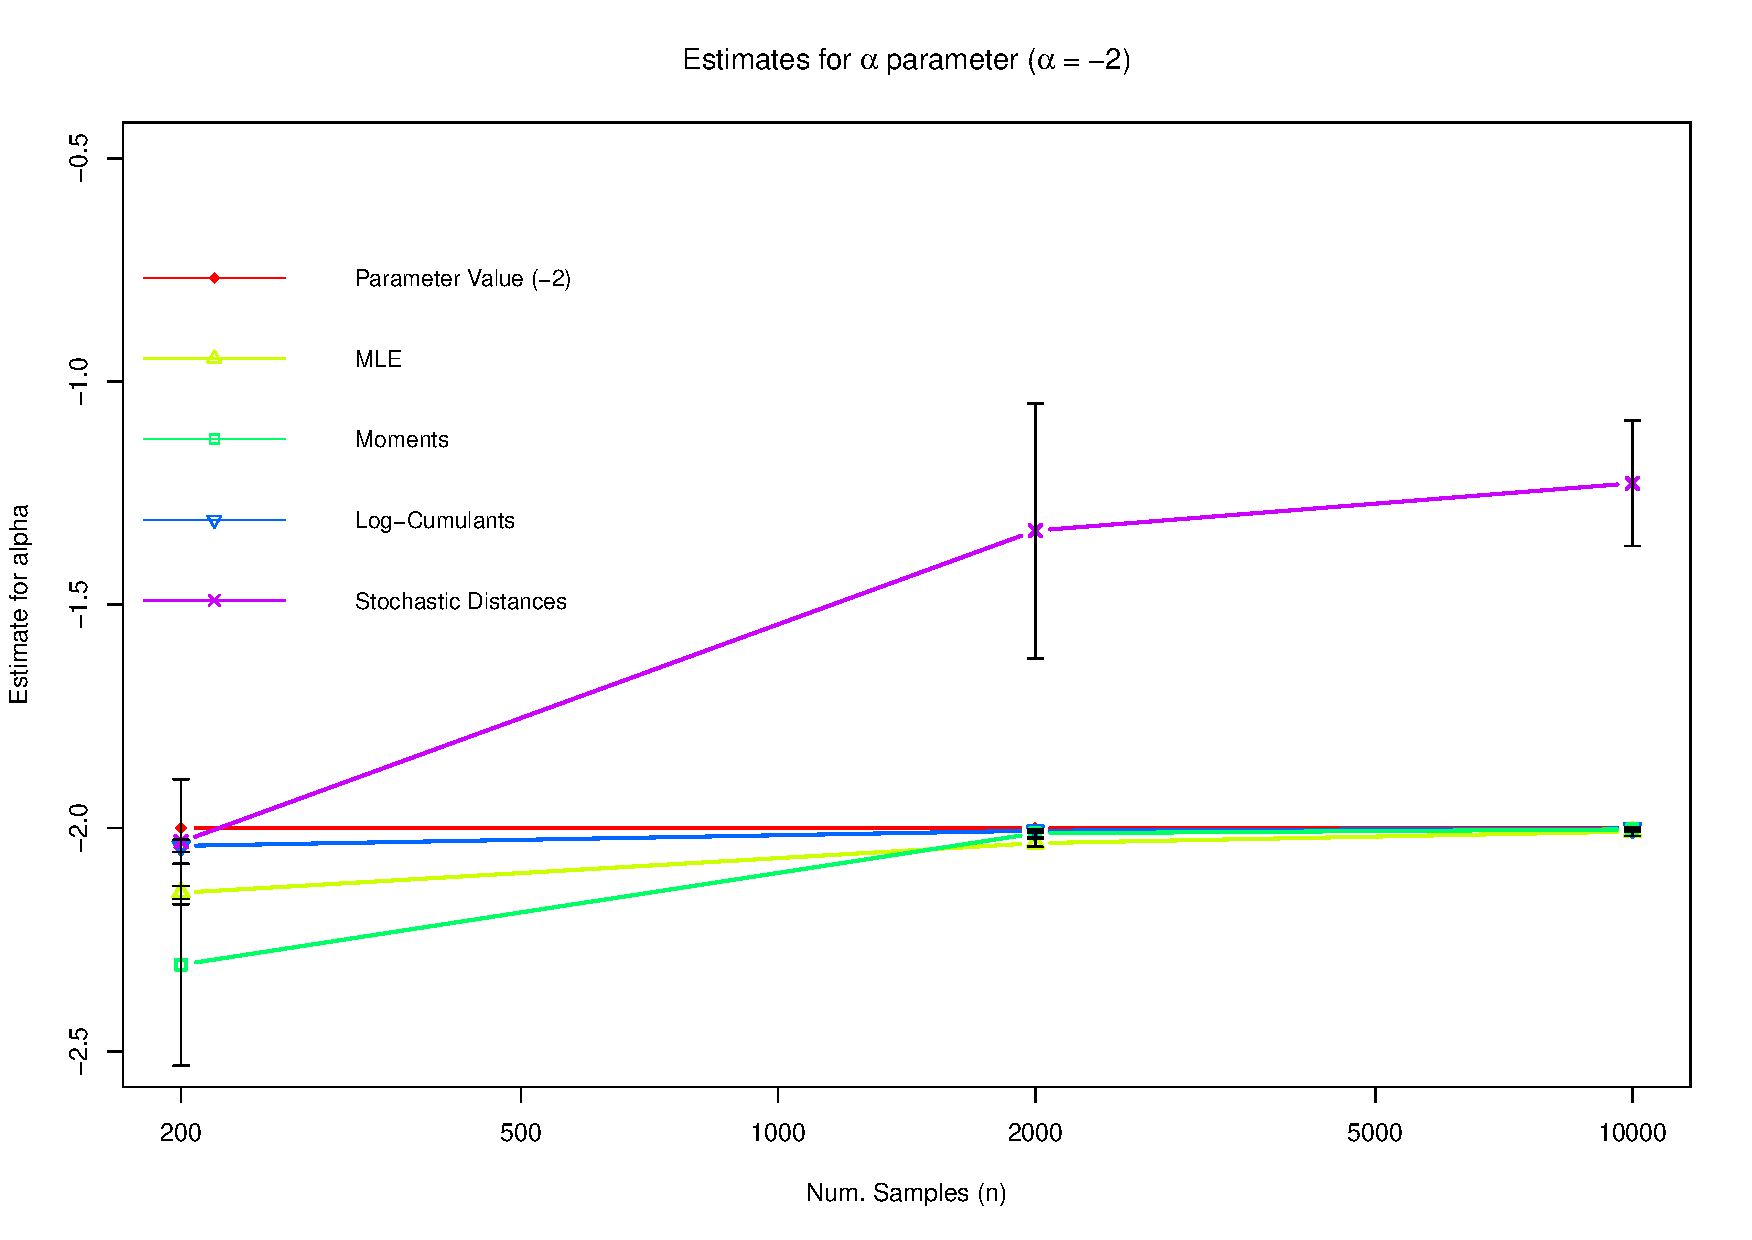
\includegraphics[scale=0.5]{plots/ComparisonAlpha-2.pdf}
     \caption{Estimativas obtidas para o parâmetro $\alpha = -2$}
     \label{graf_5}
\end{figure}
\begin{figure}[H]
     \centering
     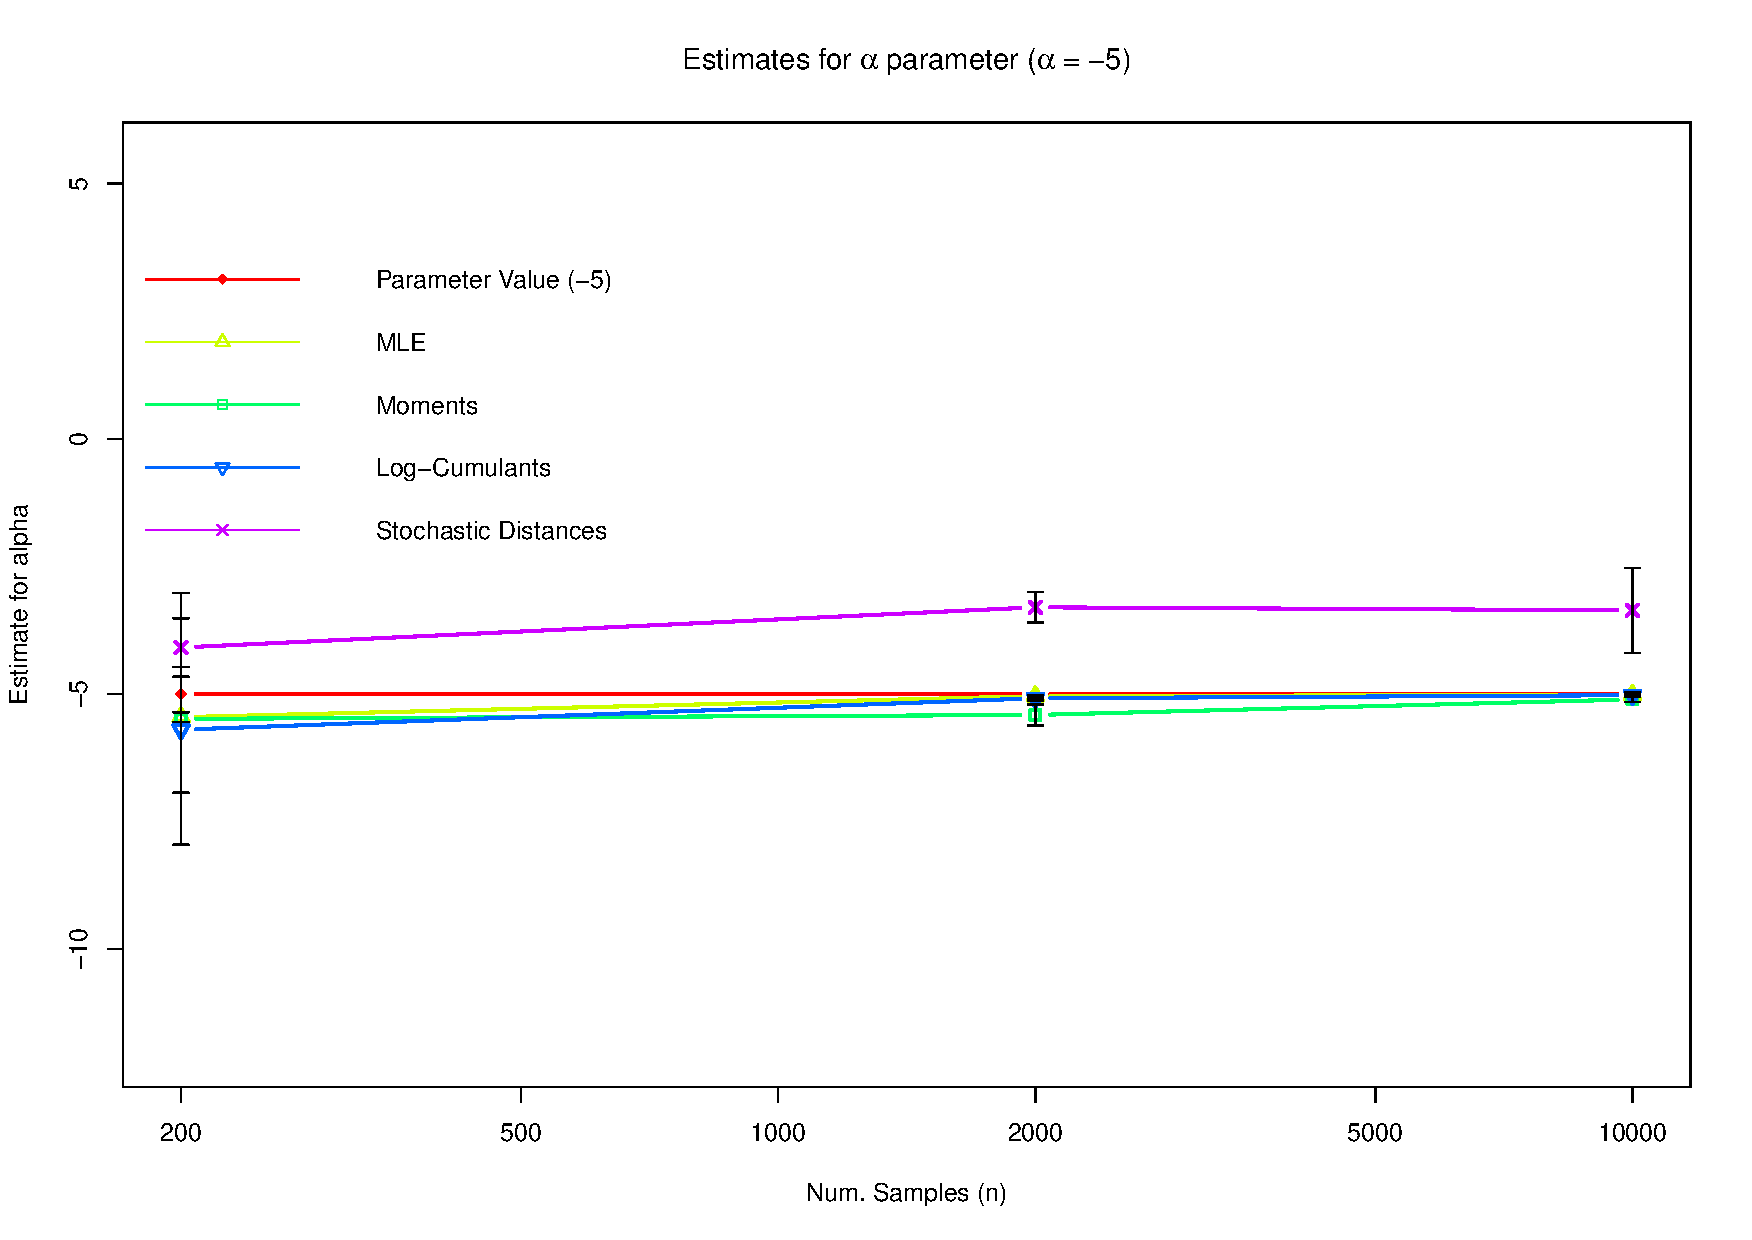
\includegraphics[scale=0.5]{plots/ComparisonAlpha-5.pdf}
     \caption{Estimativas obtidas para o parâmetro $\alpha = -5$}
     \label{graf_6}
\end{figure}
\begin{figure}[H]
     \centering
     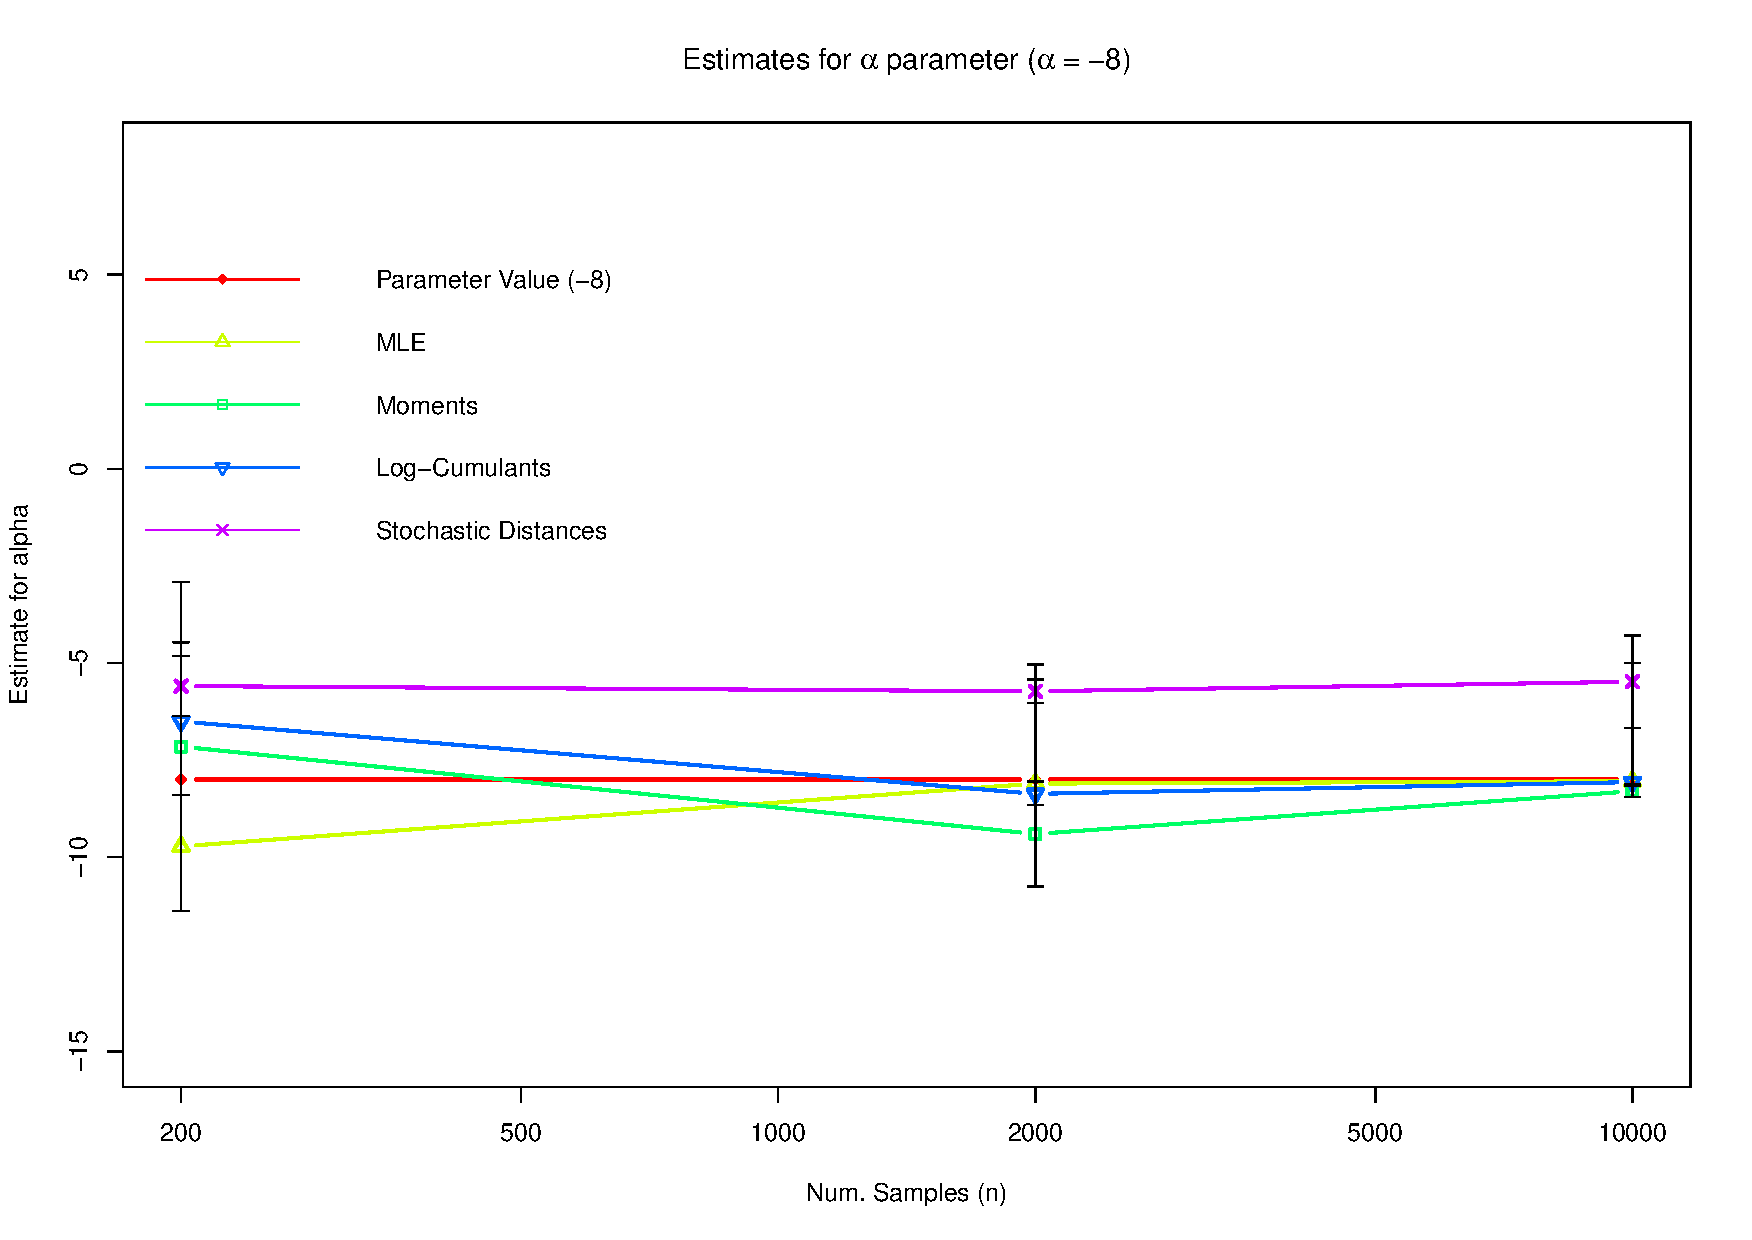
\includegraphics[scale=0.5]{plots/ComparisonAlpha-8.pdf}
     \caption{Estimativas obtidas para o parâmetro $\alpha = -8$}
     \label{graf_7}
\end{figure}

Para o estudo inicial de simulação feito, pode-se perceber através dos gráficos que os métodos de estimação conquistaram resultados satisfatórios. Em análise aos gráficos, os métodos baseados em Máxima Verossimilhança e Log-Momentos apresentaram boa capacidade de convergência para o verdadeiro valor do parâmetro à medida que o número de amostras (tamanho amostral) aumentou. No entanto, sempre pode existir uma eventual falta de convergência para o valor real do parâmetro inerente a todos os algoritmos de estimação implementados. O estimador baseado em mecanismos da Teoria da Informação, mas especificamente na Minimização de Distâncias Estocásticas, foi o que apresentou resultados mais discrepantes em relação aos demais métodos em análise aos gráficos gerados.

Entretanto, este foi apenas um estudo inicial a respeito das técnicas de estimação de parâmetros implementadas e  novos planos de simulação e investigação mais elaborados foram feitos para avaliar melhor tais técnicas, bem como analisar suas possíveis restrições e aplicações em um contexto unificado, onde existirá uma rotina de estimação geral que engloba esses métodos e seja capaz de aplicar os mais adequados para cada situação com a mínima intervenção possível do usuário tendo em vista seus pontos fortes e fracos de aplicação.

\section{Experimento II: Monte Carlo mais elaborado}

Agora nessa seção será descrito o segundo experimento de Monte Carlo que foi construído de forma mais minuciosa e elaborada de modo a possibilitar uma análise mais profunda a cerca das técnicas de estimação implementadas. Nesse contexto, temos a seguir uma tabela contendo o espaço de parâmetros utilizado nesta simulação.
\begin{table}[H]
\centering
\caption{Espaço de parâmetros utilizado na simulação mais elaborada}
\smallskip
\sisetup{table-format = 3.2}
\label{tab:tabela_parameters_2}
\begin{tabular}{c|c}
\toprule 
\multicolumn{1}{c|}{Parâmetros} & \multicolumn{1}{c}{Valores}  \\ 
\midrule
\rowcolor[gray]{.9} 
$n$ & $\{30, 100, 1000\}$ \\ \hline
$\alpha$ & $\{-1.5, -3, -8\}$ \\ \hline
\rowcolor[gray]{.9} $\gamma^*$ & $\{-\alpha - 1\}$ \\ \hline
\textit{Looks} & $\{1, 3, 5, 8\}$ \\ 
\bottomrule
\end{tabular}
\end{table}

Para realizar este experimento de Monte Carlo levou-se em consideração que amostras maiores apresentam maior variabilidade de dados em comparação com amostrar menores, então no contexto das replicações existentes no experimento definiu-se uma constante $R = 100.000$ onde o número de réplicas/repetições de amostras é dado conforme a seguinte fórmula:
\begin{equation}
    Rep = [R/n] \label{eq:rep}
\end{equation}
Nesse contexto, o número de replicações varia de acordo com cada tamanho de amostra em que amostras menores precisam ser replicadas um número maior de vezes para possibilitar a coleta de maior variabilidade dos dados, enquanto que amostras maiores não necessariamente precisam ser replicadas um número grande de vezes como no caso das amostras menores, sendo suficiente apenas um número de replicações inferior. 

Assim, os estimadores foram gerados com base nesse experimento e foram calculados e comparados tanto o viés denotado por $\widehat{B}(\widehat{\alpha}) = \alpha_i - \alpha$ quanto o erro quadrático médio para análise da acurácia. Nas figuras seguintes, "ML", "Mom", "LCum" e "DT" denotam os estimadores baseados em Máxima Verossimilhança (do inglês, \textbf{M}aximum \textbf{L}ikelihood), Momentos, Log-Cumulantes e Distância Triangular. Os tamanhos amostrais se encontram nas abscissas dos gráficos e, para uma melhor visualização, estão apresentados em uma escala logarítmica. O valor real do parâmetro está presente em cada gráfico representado pela linha de cor vermelha. Abaixo estão os gráficos gerados agrupados pelo número de \textit{Looks}.
\begin{figure}[H]
     \centering
     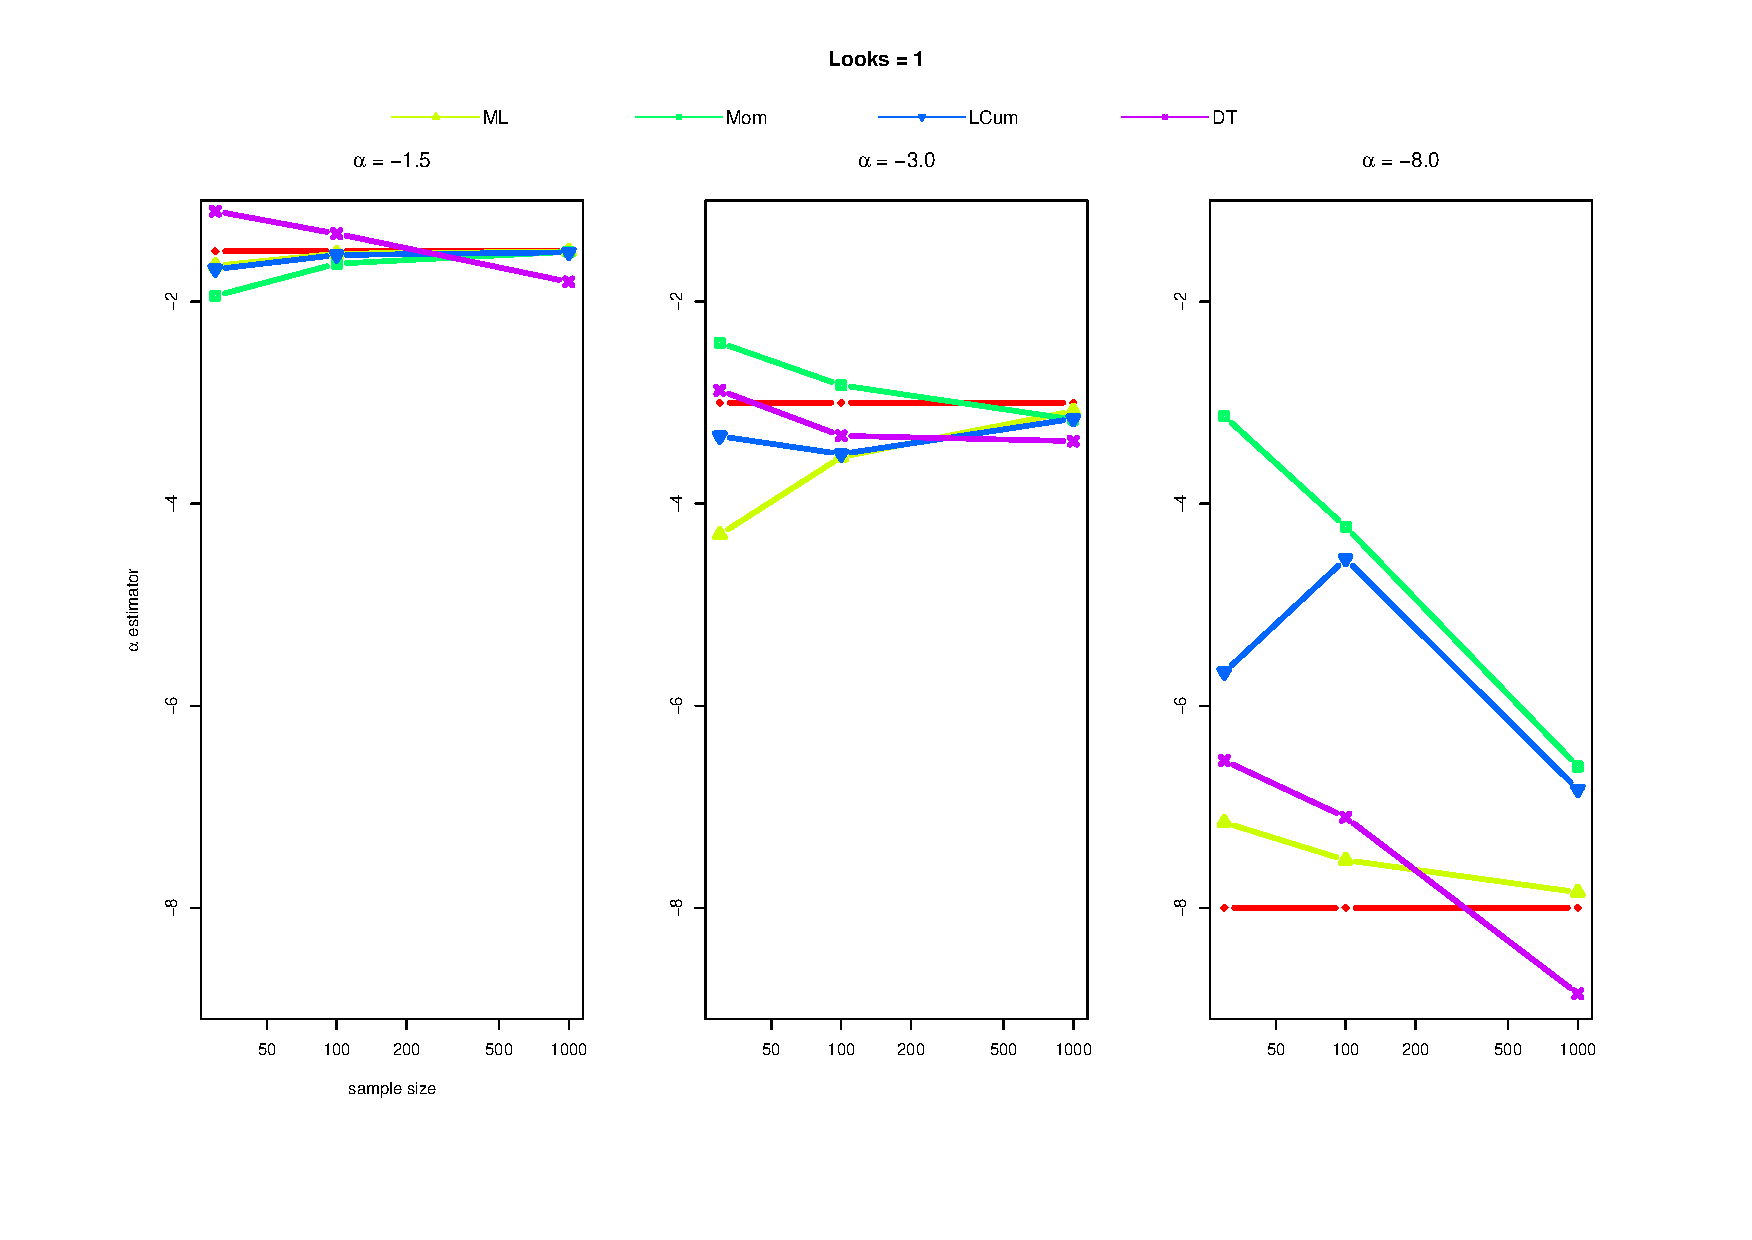
\includegraphics[scale=0.5]{plots/estimators_L=1.pdf}
     \caption{Estimativas obtidas para $L=1$}
     \label{graf_8}
\end{figure}
\begin{figure}[H]
     \centering
     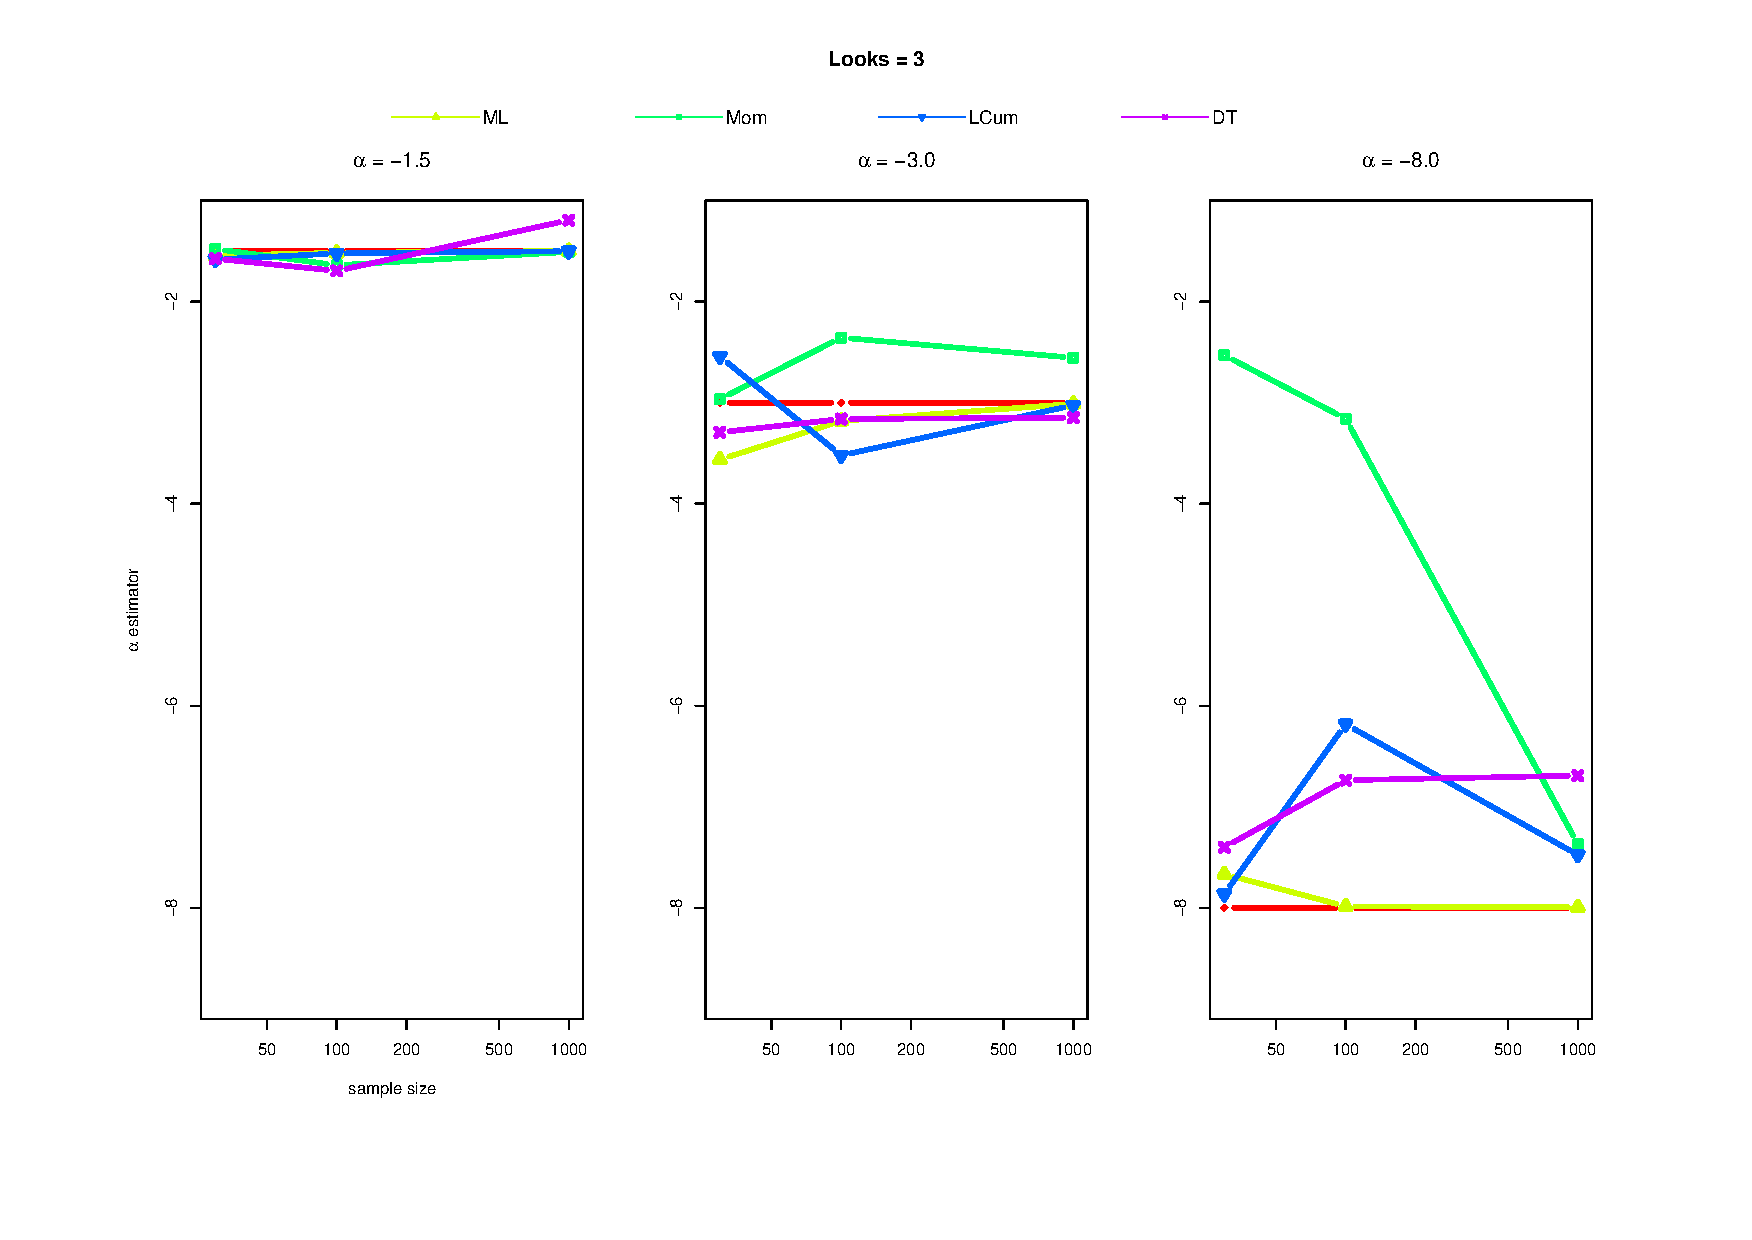
\includegraphics[scale=0.5]{plots/estimators_L=3.pdf}
     \caption{Estimativas obtidas para $L=3$}
     \label{graf_9}
\end{figure}
\begin{figure}[H]
     \centering
     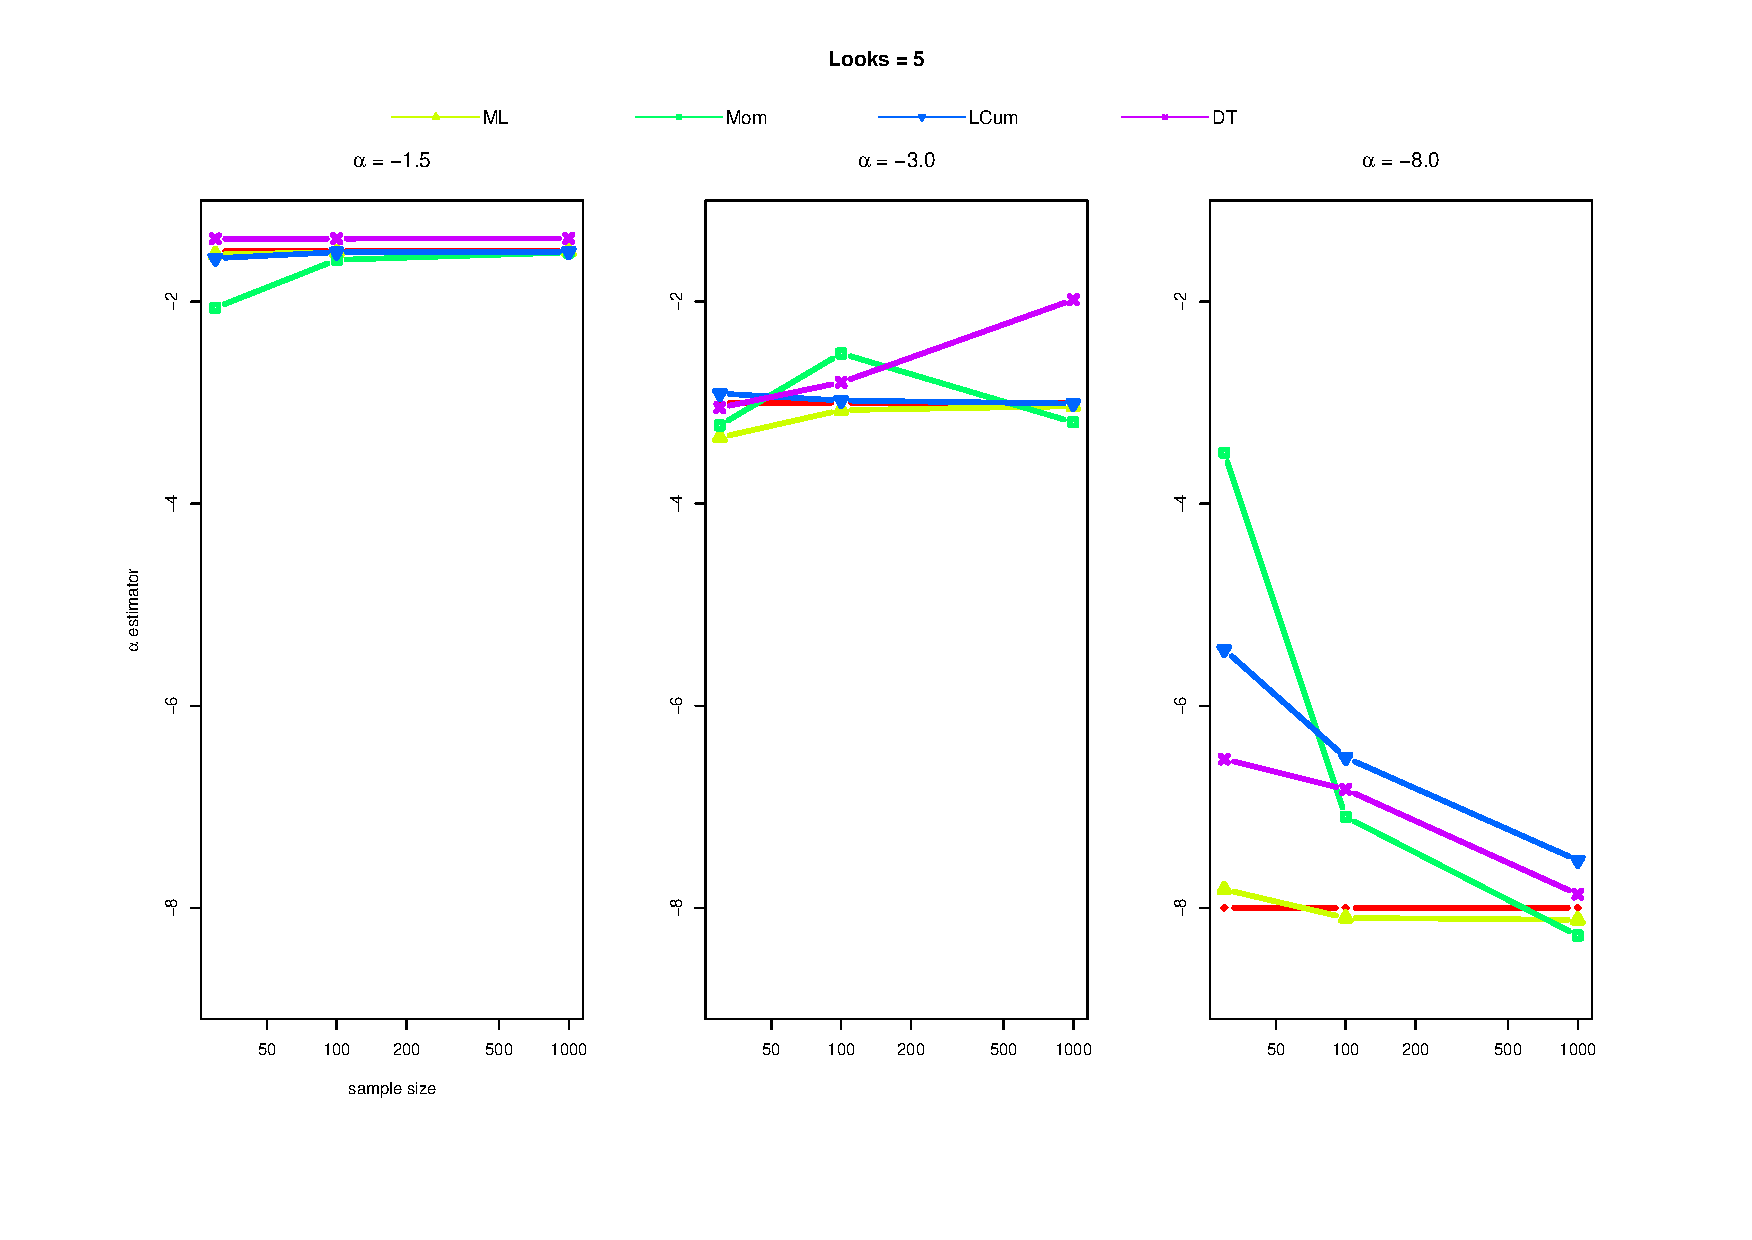
\includegraphics[scale=0.5]{plots/estimators_L=5.pdf}
     \caption{Estimativas obtidas para $L=5$}
     \label{graf_10}
\end{figure}
\begin{figure}[H]
     \centering
     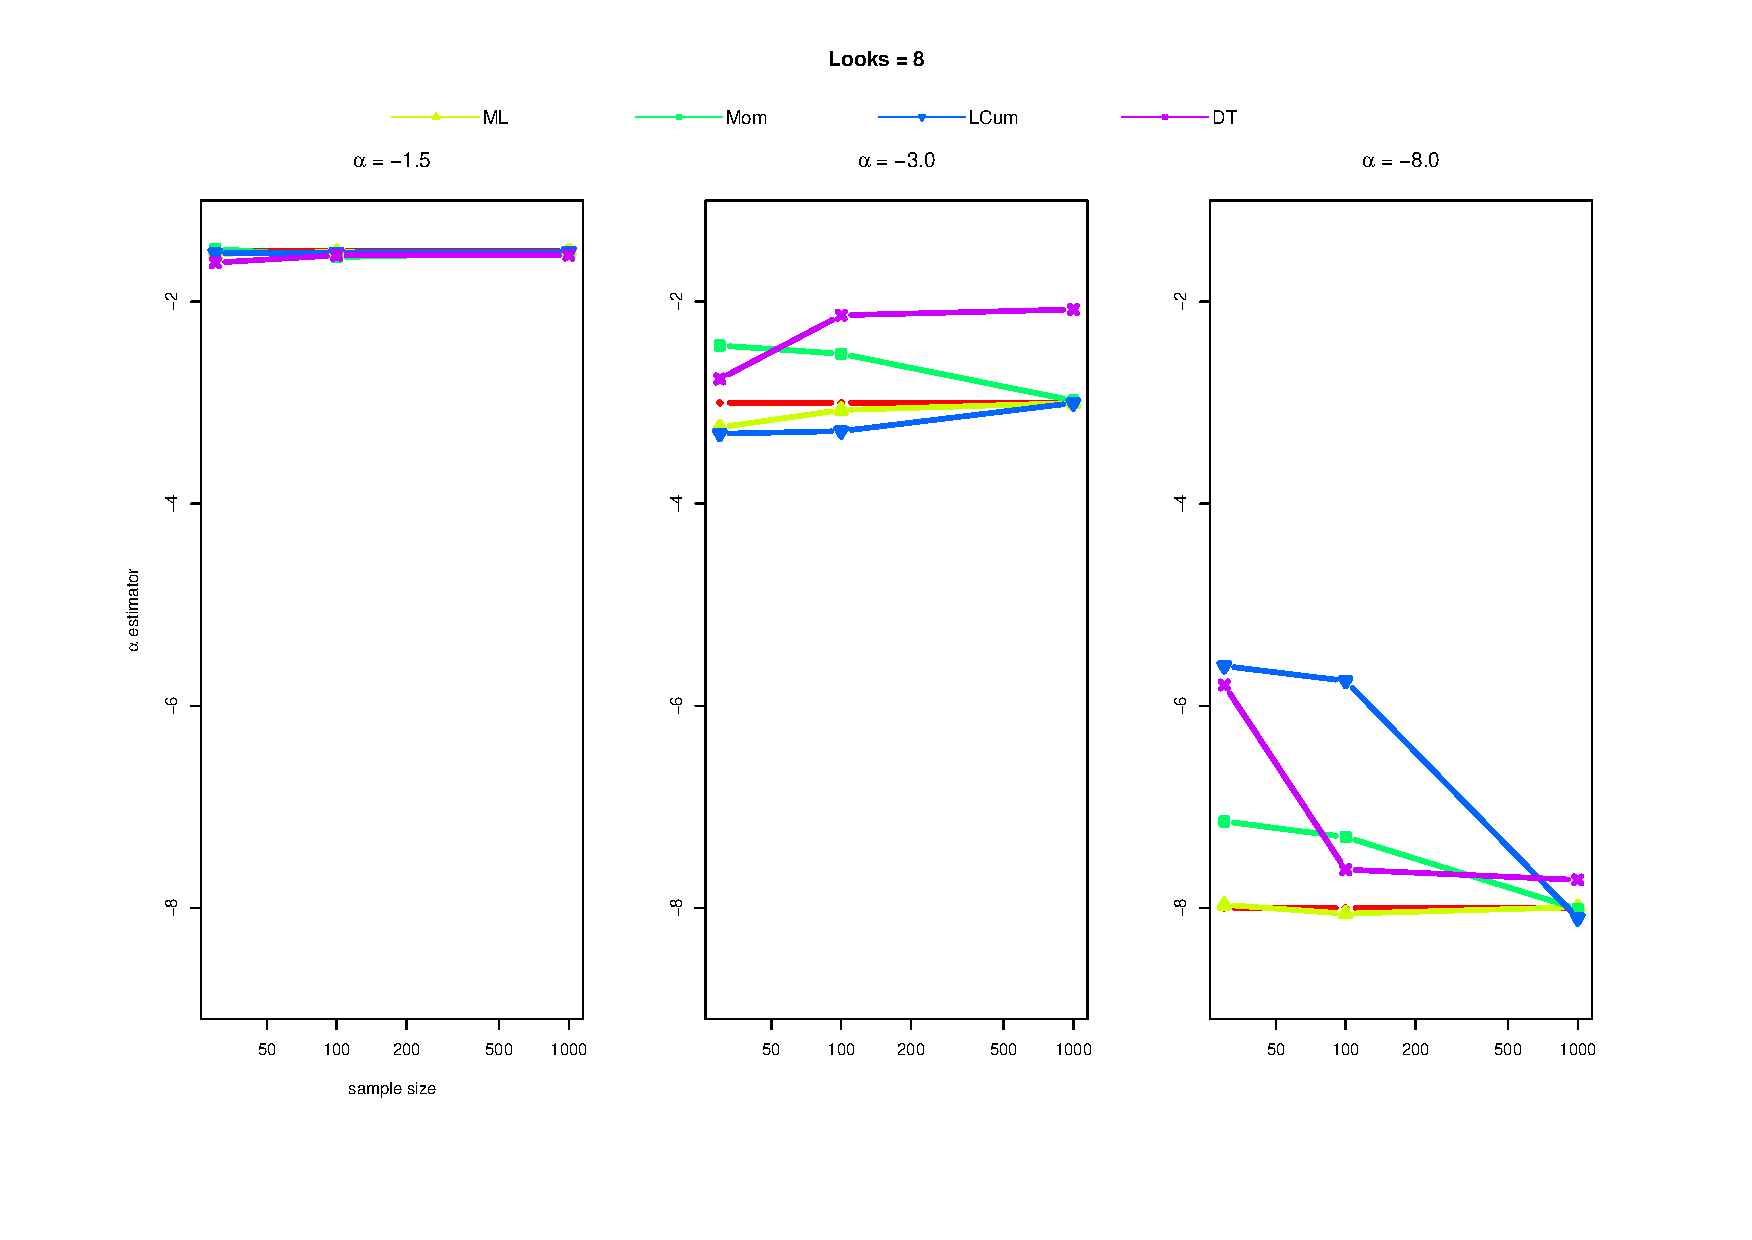
\includegraphics[scale=0.5]{plots/estimators_L=8.pdf}
     \caption{Estimativas obtidas para $L=8$}
     \label{graf_11}
\end{figure}

Abaixo agora encontram-se as figuras relativas aos erros quadráticos médios que foram calculados durante a experiência de Monte Carlo realizada. 
\begin{figure}[H]
     \centering
     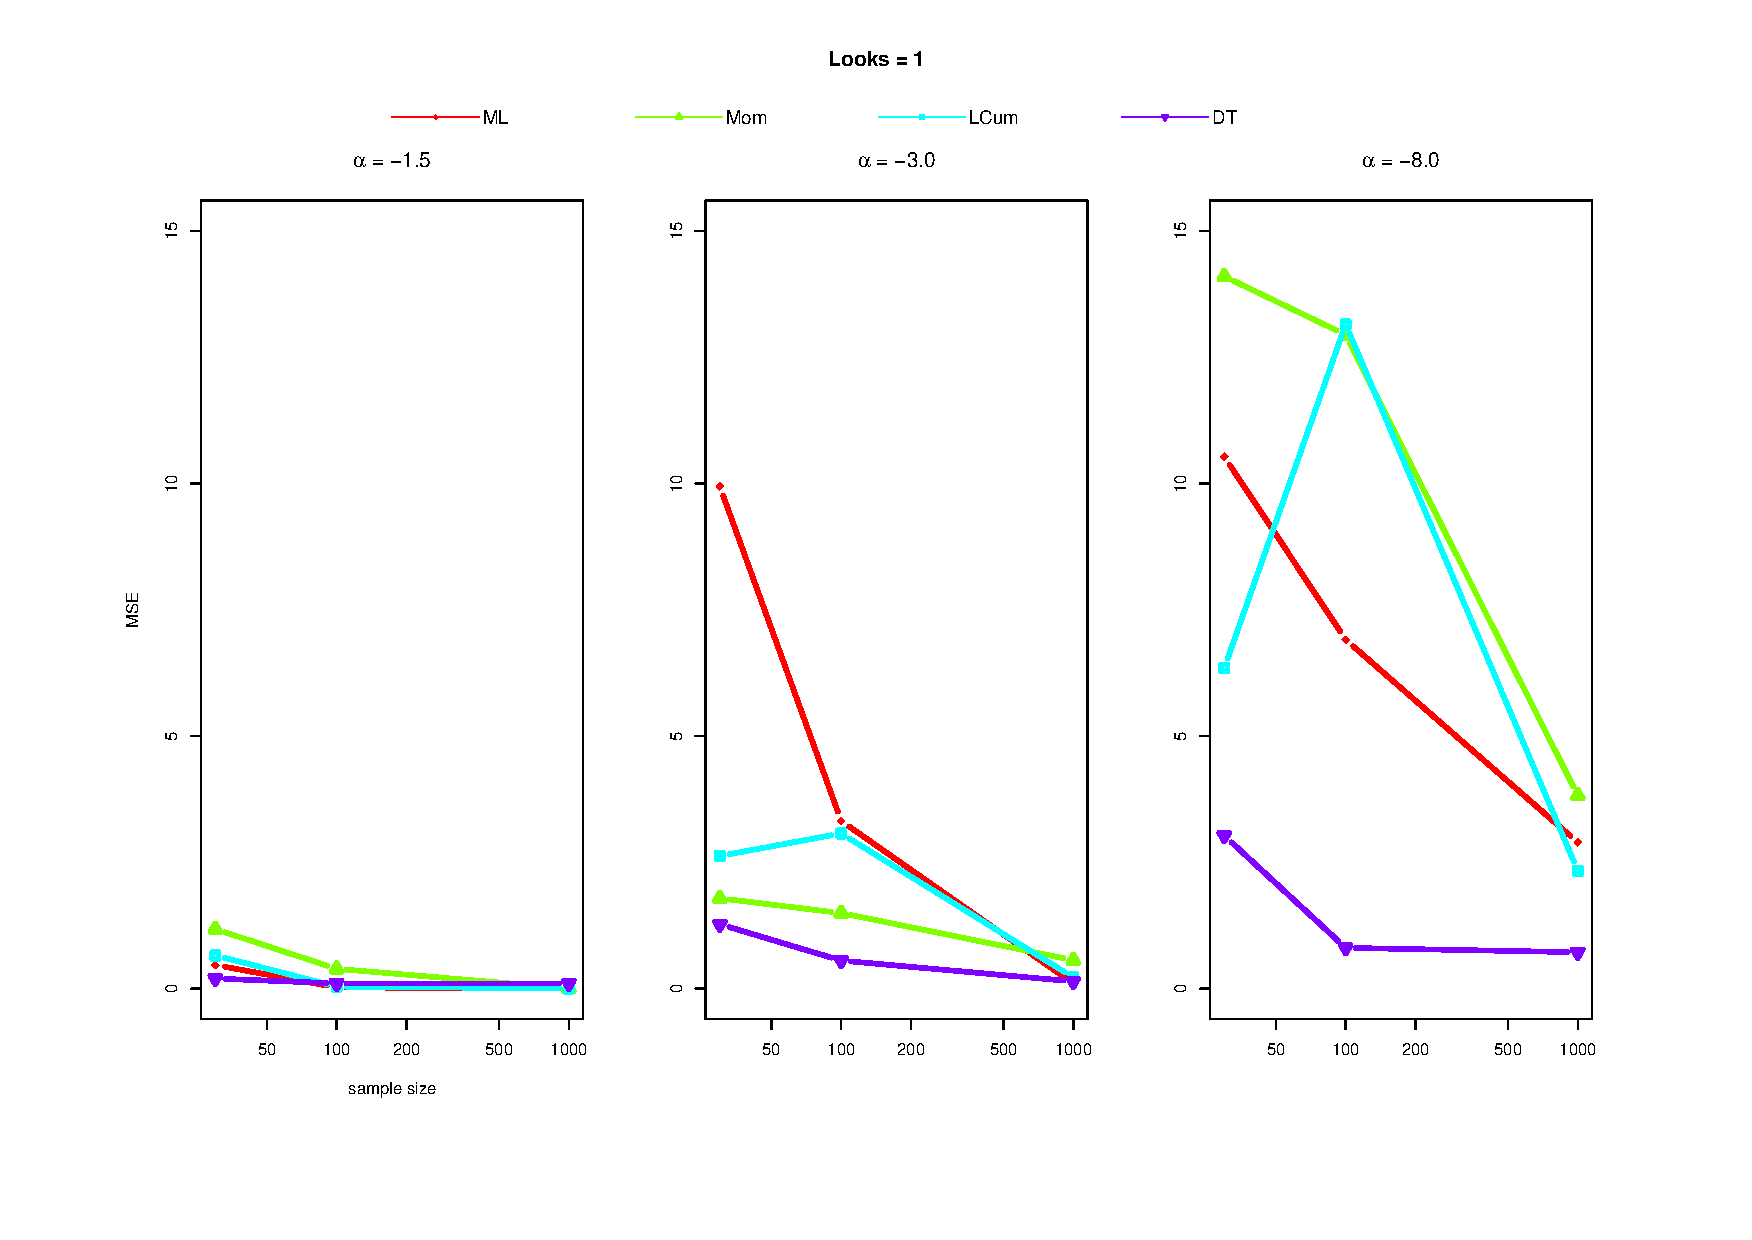
\includegraphics[scale=0.5]{plots/mse_L=1.pdf}
     \caption{Erros obtidos para $L=1$}
     \label{graf_12}
\end{figure}
\begin{figure}[H]
     \centering
     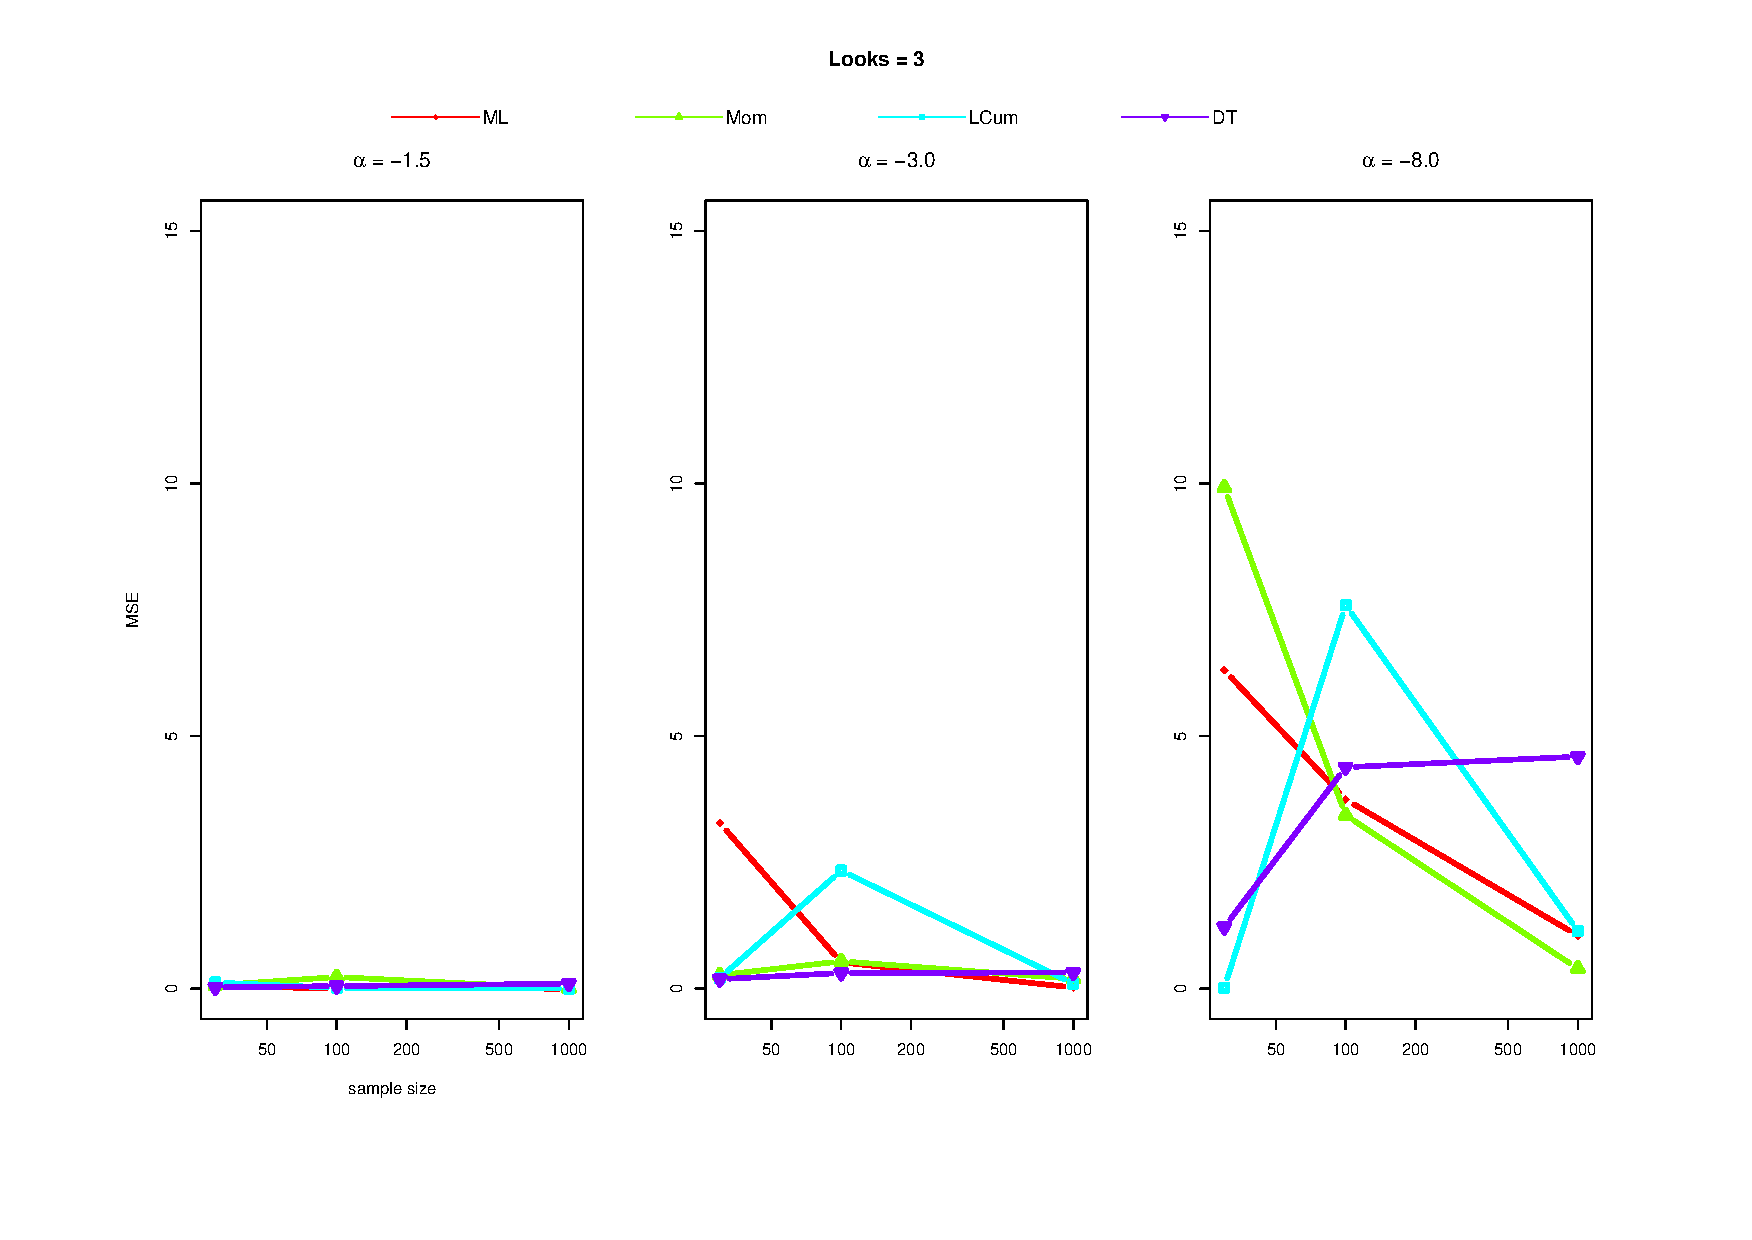
\includegraphics[scale=0.5]{plots/mse_L=3.pdf}
     \caption{Erros obtidos para $L=3$}
     \label{graf_13}
\end{figure}
\begin{figure}[H]
     \centering
     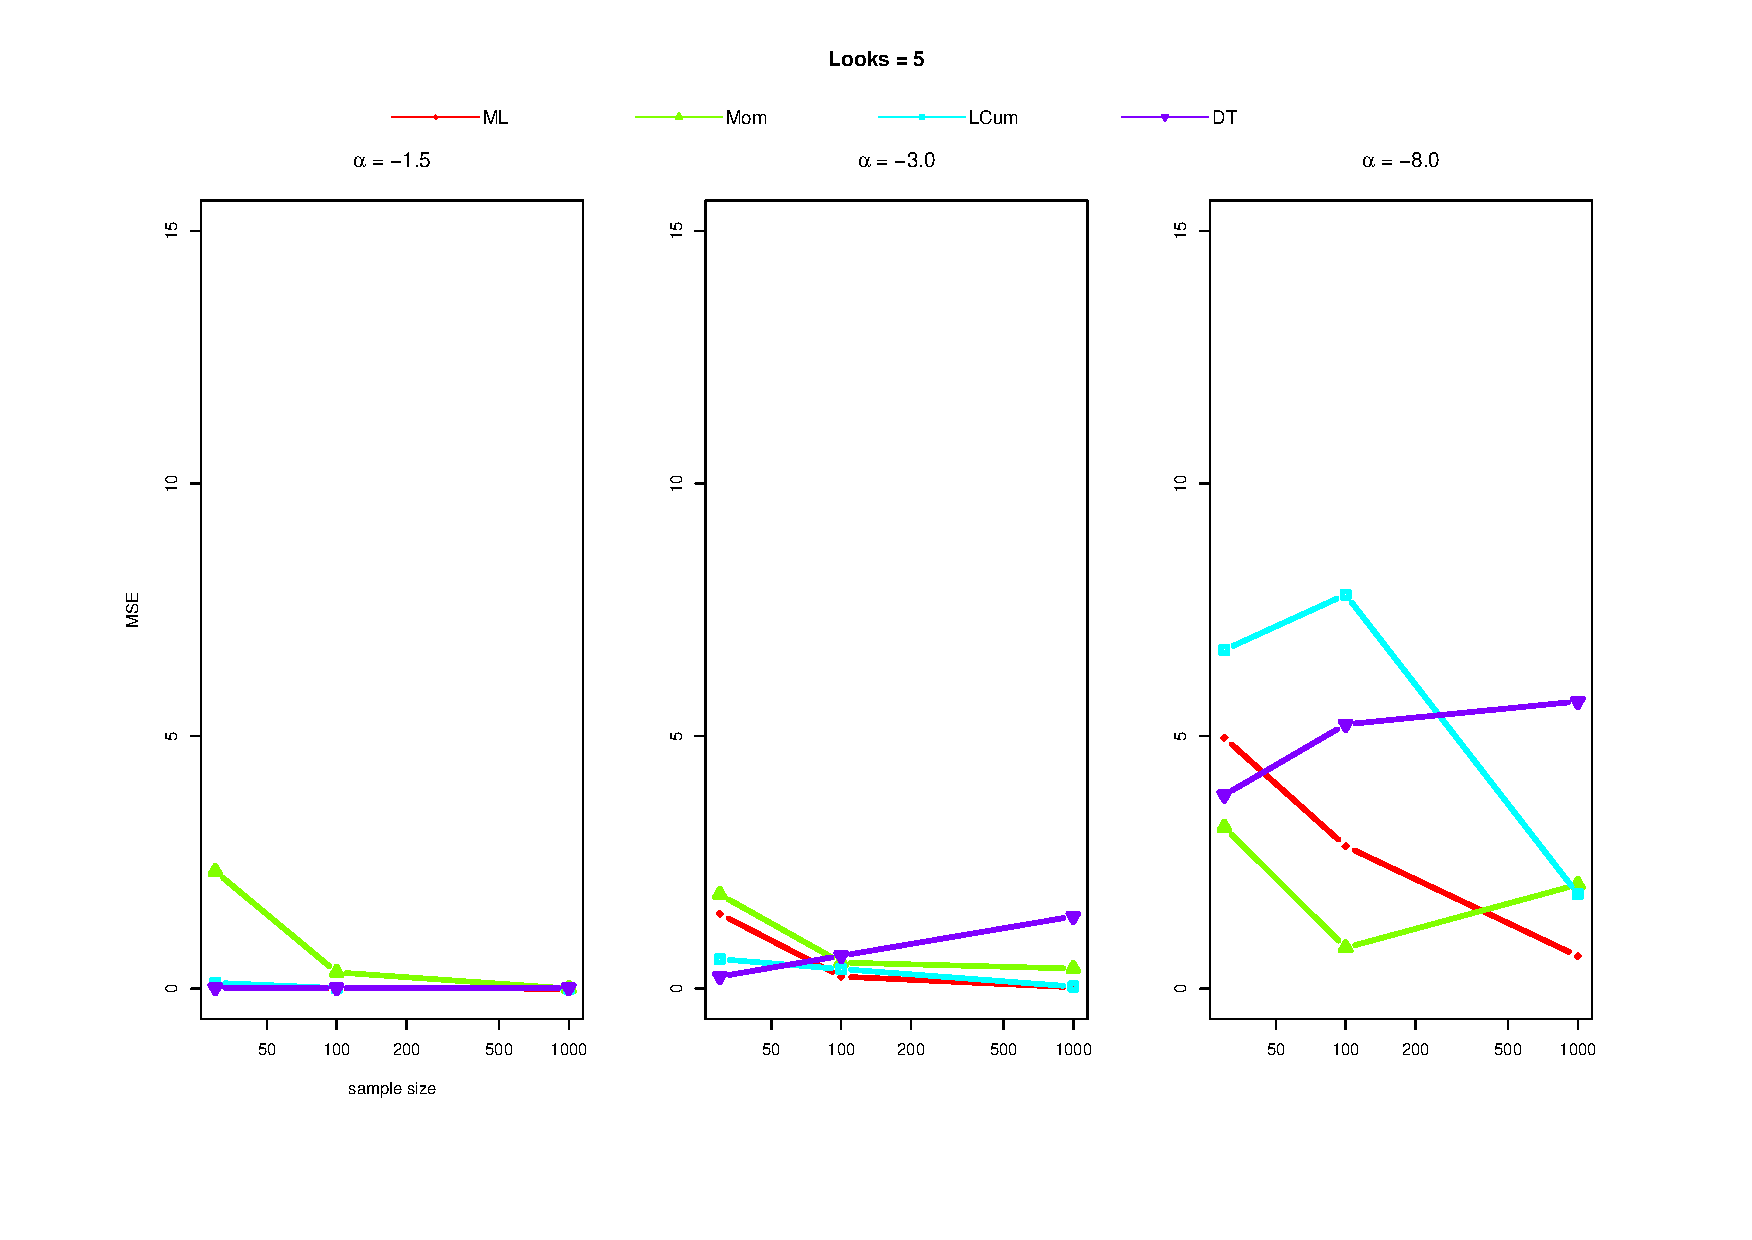
\includegraphics[scale=0.5]{plots/mse_L=5.pdf}
     \caption{Erros obtidos para $L=5$}
     \label{graf_14}
\end{figure}
\begin{figure}[H]
     \centering
     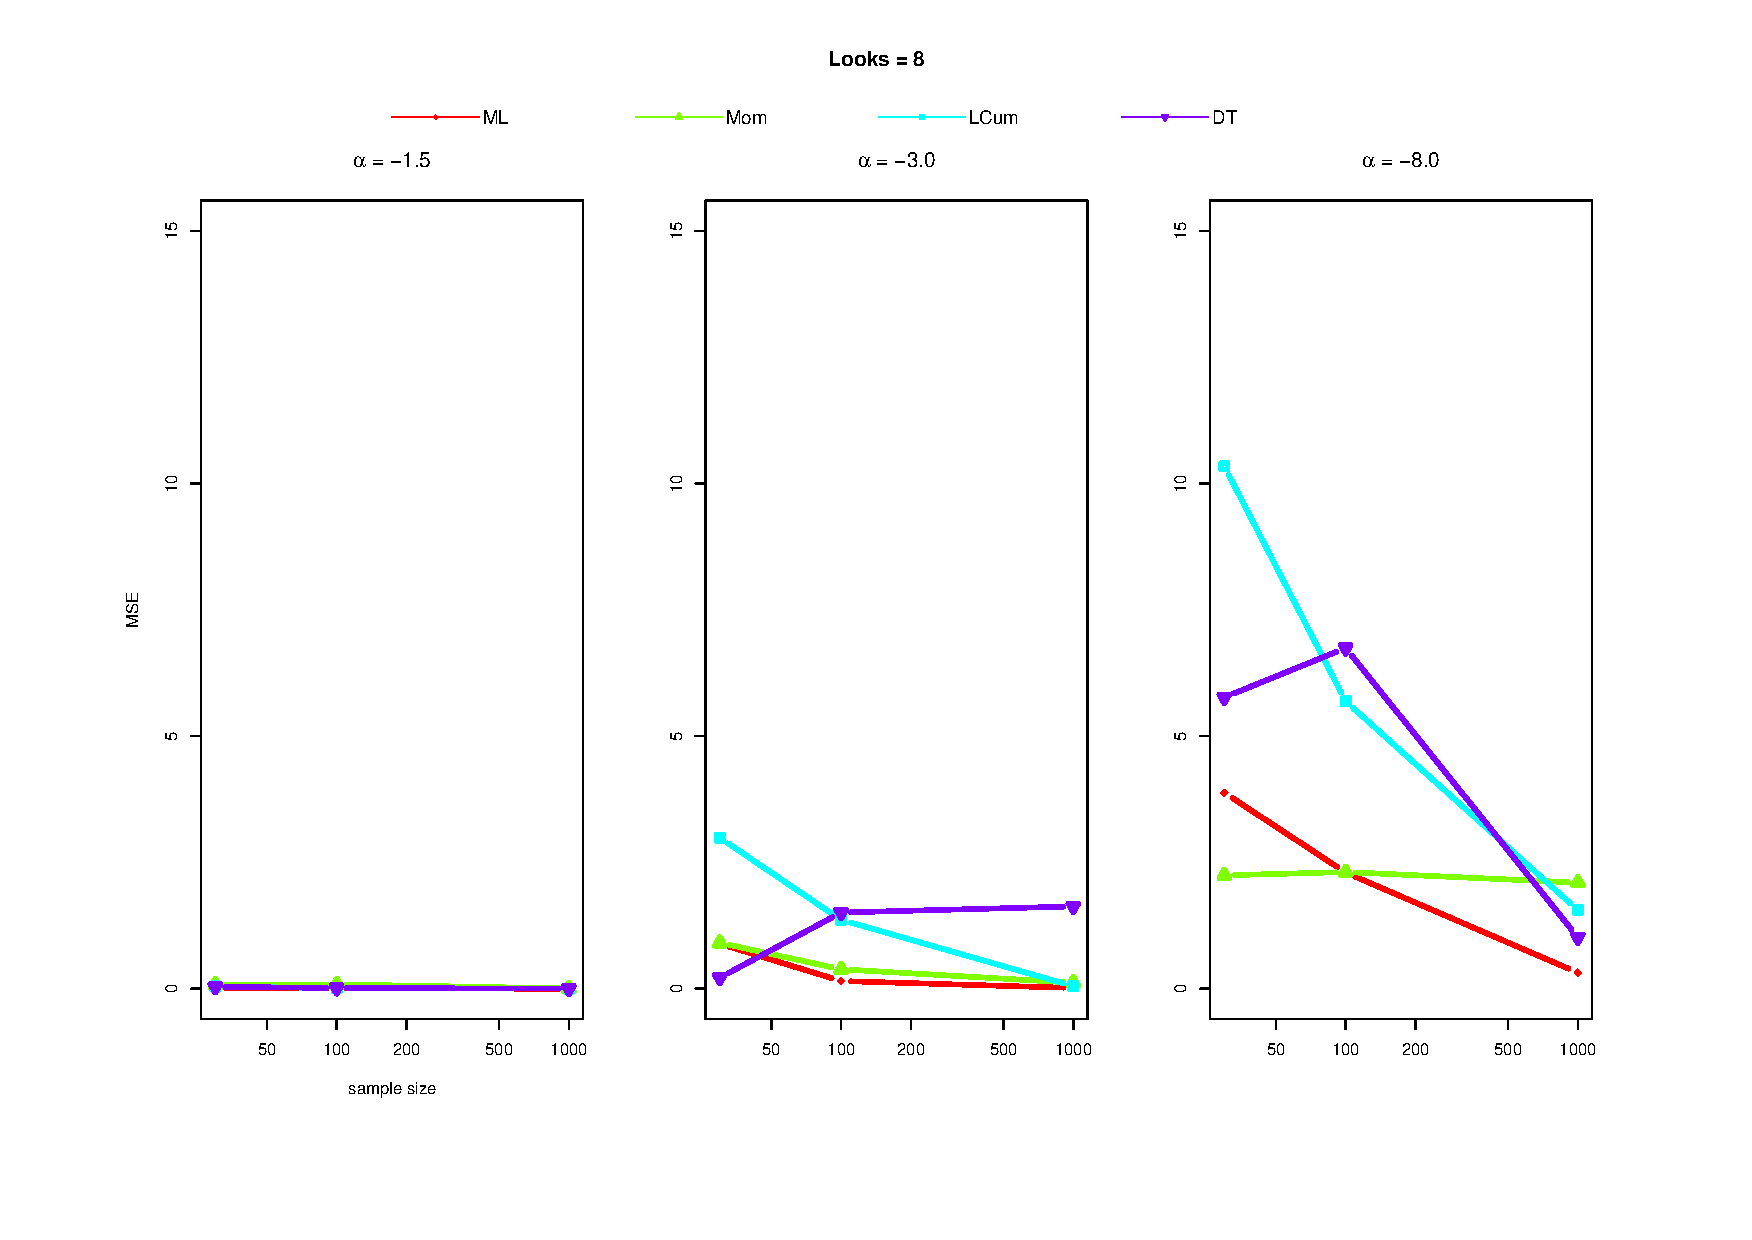
\includegraphics[scale=0.5]{plots/mse_L=8.pdf}
     \caption{Erros obtidos para $L=8$}
     \label{graf_15}
\end{figure}

Ao analisar todos os gráficos gerados, podemos perceber que duas técnicas de estimação apresentam, em média, estimadores muito próximos do valor verdadeiro: Máxima Verossimilhança e Distância Triangular. Os gráficos ainda mostram que para valores de $\alpha$ cada vez menores, independentemente do número de \textit{Looks}, as estimativas vão se tornando cada vez discrepantes em relação ao valor verdadeiro. É bastante notável a discrepância dos estimadores de Momentos e Log-Cumulantes quando $\alpha = -8$, e, mais especificamente, quando $L = 1$. 

Não obstante, é perceptível que $\alpha_{ML}$ tem uma tendência sistemática para subestimar o verdadeiro valor de $\alpha$. Além dessas observações, vale salientar que para o valor de $\alpha = -1.5$ as estimativas providas por todas as técnicas se mostraram bem próximas do valor verdadeiro do parâmetro em questão. \citet{FreryStochasticDistances2015} calcularam uma aproximação de primeira ordem de tal viés para um modelo estreitamente relacionado, e os resultados obtidos aqui estão de acordo com aqueles.

Vale ressaltar ainda que há possibilidade de uma eventual falta de convergência inerente a todos os algoritmos de estimação, visto que nem sempre tais algoritmos são extremamente precisos no cálculo e/ou podem falhar resultando em estimadores bem discrepantes do valor real ou simplesmente não conseguir encontrar a solução, devido, por exemplo, a não existência de raízes das equações lineares que os algoritmos de Momentos e Log-Cumulantes utilizam ou a falha na otimização dos algoritmos de Máxima Verossimilhança e Distância Triangular.

Ademais, nas figuras acima, onde estão mostrados os gráficos com os erros quadráticos médios referentes à cada técnica de estimação, pode-se perceber que, na maioria dos casos, todos os estimadores têm erro quadrático médio (\textit{mse - mean square error}) muito semelhante, não sendo possível afirmar com certeza que um deles é sistematicamente o melhor que o outro. O que pode ser feito é analisar onde cada estimador pode ser melhor aplicado observando os casos em que os mesmos obtiveram os melhores resultados e possuem menores chances de fornecer más estimativas. É baseado nessa ideia de construção de um algoritmo de estimação integrado com todos os algoritmos de estimação que esse trabalho propôs a criação de uma rotina de estimação unificada que encapsula diversos desses métodos e seja capaz de escolher o melhor para cada caso que lhe aparece. Essa rotina será melhor explicada na seção seguinte.

\section{Rotina de Estimação Unificada}

\subsection{Considerações iniciais}

Esta seção visa abordar o funcionamento geral da rotina de estimação que encapsula os algoritmos de estimação implementados e tem autonomia para tomar alguma decisão e executar alguma das técnicas desenvolvidas, diante de cada situação prevista. 

Com base nos experimentos de Monte Carlo que foram realizados foi possível fazer uma avaliação geral da qualidade de cada técnica implementada analisando o desempenho de cada uma delas em diferentes cenários considerando diferentes números de \textit{Looks}, diferentes graus de textura da imagem - homogênea, heterogênea ou extremamente heterogênea - e diferentes tamanhos de amostra. O funcionamento de tal rotina de estimação foi pensado com base na análise de estudos feitos na literatura e, sobretudo, com base nos experimentos realizados.

Na subseção seguinte temos o fluxograma do funcionamento geral da rotina de estimação implementada, bem como algumas explicações e diretrizes, escritas em detalhes, que foram tomadas para a sua construção. 

\subsection{Fluxograma de Execução da Rotina de Estimação}

Abaixo encontra-se o fluxograma de execução propriamente dito. Como pode-se perceber, a rotina de estimação desenvolvida é tolerante a falhas. Tolerância a falhas é a propriedade que permite que sistemas computacionais ou outros tipos de sistemas continuem a operar normalmente mesmo após ocorrência de falhas em alguns de seus componentes, seguindo, nesse caso, um fluxo de execução alternativo. Nesse sentido, a rotina desenvolvida sempre vai tentar retornar para o usuário um valor para o estimador, independente de falha em algum algoritmo, a não ser que a entrada de dados definida por ele seja inválida. O seguinte raciocínio foi levado em consideração para a construção desse fluxograma:
\begin{itemize}
    \item No início temos a interação com o usuário onde o mesmo tem a opção de escolher um algoritmo em especial para executar a estimação ou então não indicar opção alguma e deixar o sistema escolher a mais apropriada para cada caso.
    \item Se foi escolhido um algoritmo específico, o sistema vai tentar executar esse algoritmo e, se não ocorrer falhas, retorna o estimador calculado. Se houver falha, o sistema também saberá como agir verificando o tamanho da amostra e seguindo adiante até a execução de outro estimador.
    \item Se não foi escolhido um algoritmo específico ou se houver falha no passo anterior, há a verificação do tamanho da amostra da entrada. Se $n < 200$, parte-se para o método de Log-Cumulantes que se mostrou apropriado para trabalhar com amostras pequenas. O sistema vai tentar executar esse método e, se não houver falhas, retorna o estimador calculado. Se houver falha, parte-se para a verificação do número de \textit{Looks} e o sistema segue adiante até a execução de outro estimador.
    \item Se o tamanho da amostra for maior ou igual que 200 ($n >= 200$) ou se houver falha no passo anterior, há a verificação do número de \textit{Looks}. No caso em que $Looks <= 5$ executa-se a estimação por Máxima Verossimilhança que forneceu resultados bem precisos nesse caso e o estimador é calculado, se não houver falhas. Se falhar, parte-se para a verificação da textura da região.
    \item No caso em que temos $Looks > 5$ ou se houver falha no passo anterior, faz-se a verificação da textura por meio do parâmetro $\alpha$. A estimação por Distâncias Estocásticas utiliza métodos de minimização que são mais estáveis e possuem menor erro nos casos em que temos um número grande de \textit{Looks} e valores próximos de zero do parâmetro $\alpha$ que correspondem a regiões extremamente rugosas da imagem, conforme aborda \citet{Cassetti2013} em seu trabalho. Assim, o sistema vai tentar executar esse algoritmo de Distâncias Estocásticas e exibir o resultado. Se houver falhas, parte-se para o método dos Momentos. 
    \item Por sua vez, o método dos momentos vai ser executado no caso em que o parâmetro $\alpha <= -3$ ou se houver falha no passo anterior e, caso não ocorra falhas, o resultado será exibido. Se houver falhas, executa-se a estimação pelo algoritmo de Máxima Verossimilhança (foi o que apresentou os melhores resultados no geral) e exibe-se o resultado. Se esse algoritmo falhar, exibe-se a mensagem de erro para o usuário e solicita-se para o mesmo tentar novamente com dados válidos.
    
\end{itemize}
\begin{figure}[H]
     \centering
     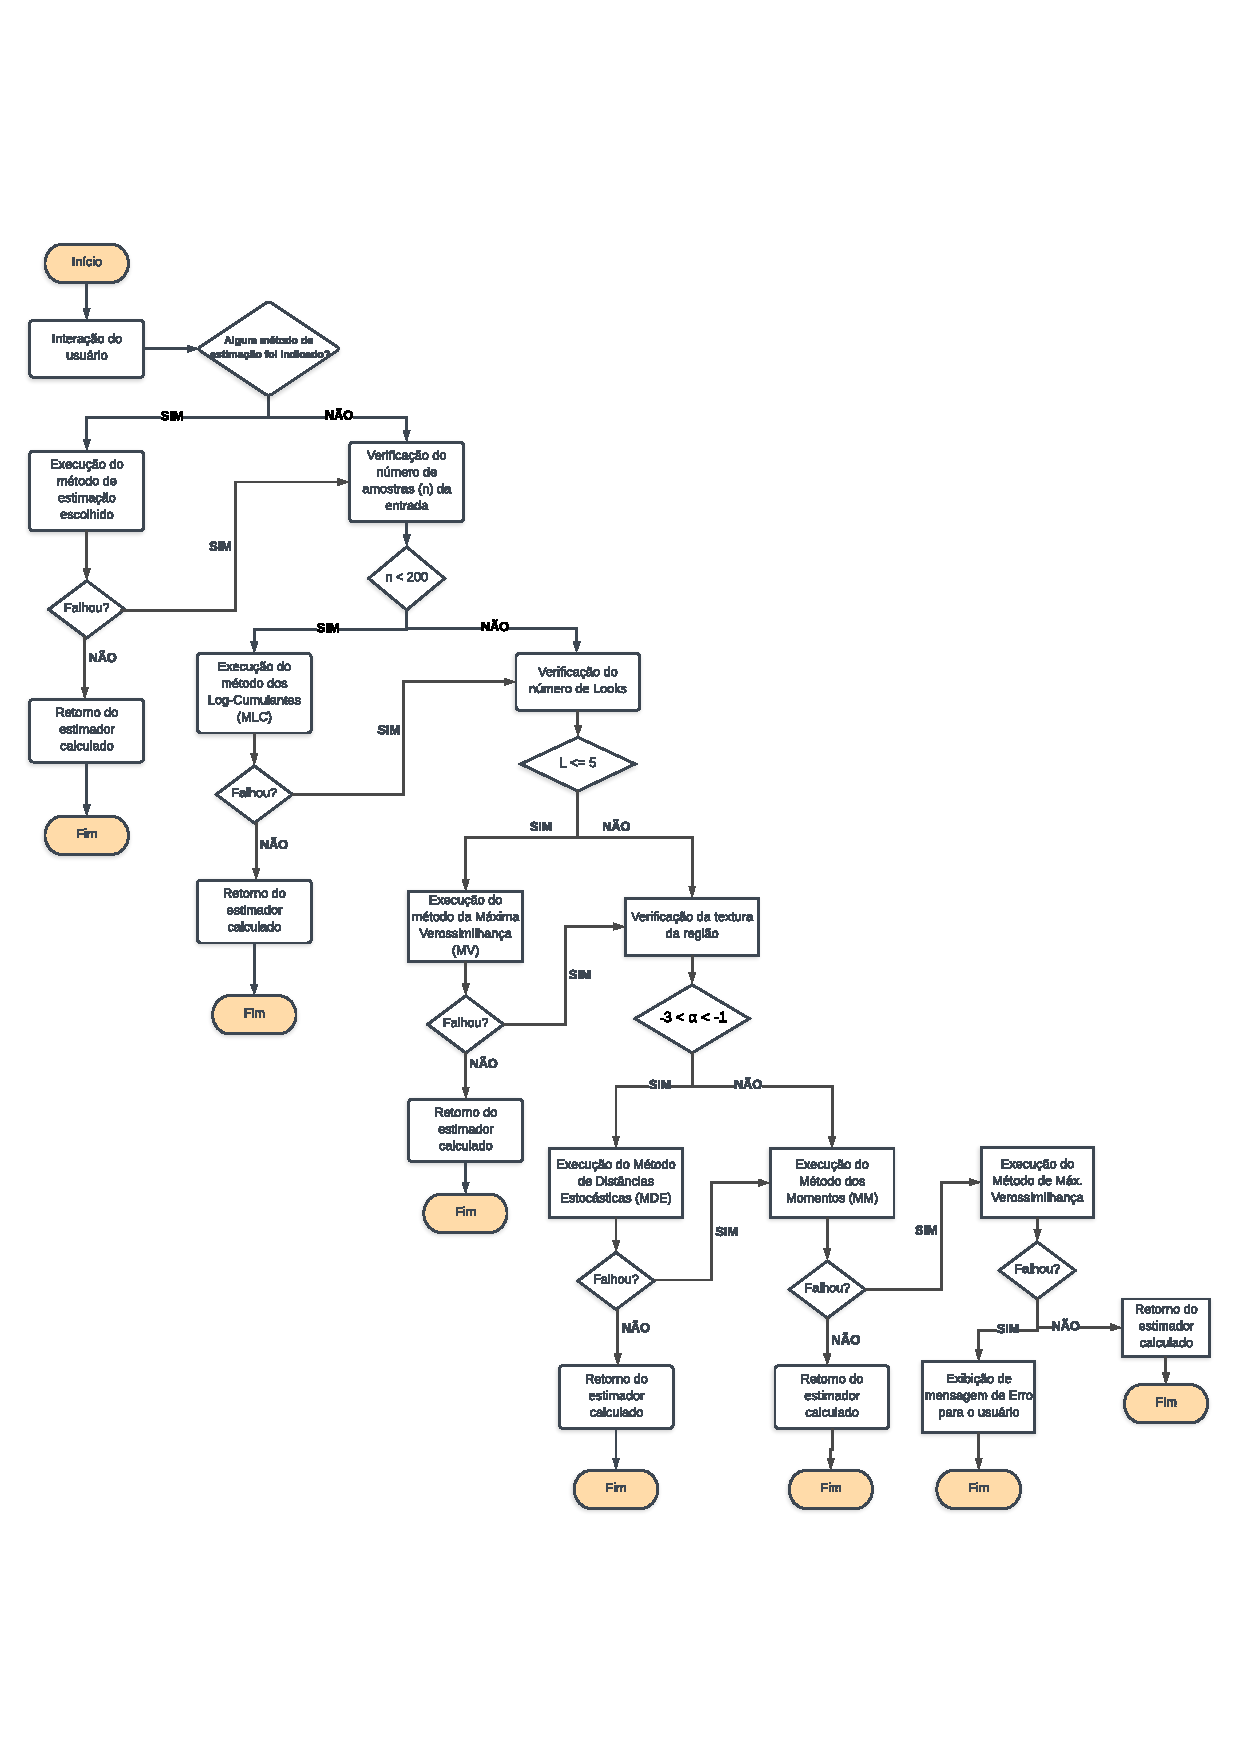
\includegraphics[scale=0.80]{plots/FluxogramaDeExecucao-A4.pdf}
     \caption{Fluxograma de execução da rotina de estimação}
     \label{fig1}
\end{figure}


\mychapter{Conclusões}{cap:conclusoes}

Neste capítulo serão abordados os avanços no meio científico e a importância proporcionada através do desenvolvimento deste trabalho. Além disso, também serão apresentadas sugestões para trabalhos futuros.

\section{Considerações Finais}

Este trabalho propôs o desenvolvimento de uma biblioteca de funções para simulação e, essencialmente, para inferência estatística em modelos para imagens SAR. O modelo trabalhado para os dados SAR foi dado pela distribuição $G_I^0$. Do ponto de vista de simulação, a principal contribuição se deu por intermédio da implementação de funções de geração de variáveis aleatórias que seguem a distribuição $G_I^0$ e de visualização gráfica da curva de sua função de densidade de probabilidade, como exibido nas figuras \ref{graf_densGI0} e \ref{graf_genGI0} do capítulo \ref{cap:fundamentacao}.

Por outro lado, do ponto de vista da inferência estatística a contribuição relevante deste trabalho se deu por meio da construção de uma rotina de estimação unificada que encapsula um total de quatro algoritmos de estimação de parâmetros (Máxima Verossimilhança, Momentos, Log-Cumulantes e Distâncias Estocásticas) e que segue um fluxograma de execução adaptativo a depender de cada caso que lhe aparece, como mostrado no capítulo anterior. Essa rotina de estimação foi elaborada pensando-se no usuário final, visto que o mesmo pode interagir com a mínima intervenção possível. A mesma aproveita o melhor de cada uma das técnicas de estimação implementadas, pois irá executar o algoritmo mais apropriado para cada caso e, dessa forma, a probabilidade de retornar estimativas precisas para o usuário final é bastante elevada.

\section{Trabalhos futuros}

Como sugestões de trabalhos futuros, pode-se pensar em uma análise profunda a cerca da forma de trabalho dos usuários finais e integrar as soluções em ferramentas provendo uma interface mais amigável, como por exemplo, utilizando alguma biblioteca gráfica compatível com a linguagem \texttt{R}. 

Ademais, alguns dos objetivos planejados para serem atingidos futuramente com este trabalho estão elencados a seguir:
\begin{itemize}
    \item Implementar uma extensão do presente trabalho considerando também os casos em que as variáveis aleatórias não são independentes e igualmente distribuídas (iid). Dessa forma, o foco seria direcionado para técnicas de estimação resistentes à \textit{outliers}, como, por exemplo, a própria técnica baseada em distâncias estocásticas, estimadores robustos \citep{Wang2017}, estimadores $M$ e $AM$ \citep{AllendeFreryetal:JSCS:05}, dentre outros existentes na literatura.
    \item Expandir o uso da rotina de estimação a fim de analisar o desempenho, acurácia e robustez dos algoritmos de estimação integrados com dados reais provenientes de imagens SAR disponíveis no site \citet{PoISARpro};
    \item Realizar testes com usuários finais para validação da ferramenta desenvolvida e dos resultados obtidos na prática.
\end{itemize}

\selectlanguage{portuguese}
\appendix
\chapter{Manual de utilização das funções desenvolvidas} \label{apendiceA}

\section{Pacotes necessários}

Para que seja possível utilizar plenamente as funções desenvolvidas ao longo deste trabalho será necessário que os seguintes pacotes estejam instalados no ambiente \textit{RStudio}:

\begin{itemize}
    \item stats4
    \item rootSolve
    \item cubature
\end{itemize}

Após a instalação, o usuário pode realizar normalmente as chamadas das funções implementadas.

\section{Principais funções desenvolvidas}

%------------------------------------------------------------------------------------------------------------------

Basicamente três funções principais foram desenvolvidas neste trabalho: \textit{densGI0}, \textit{randGI0} e \textit{estimationGI0}. Não estão listadas aqui as funções auxiliares ou subfunções utilizadas para desenvolvimento dessas funções principais, como, por exemplo, na macro função \textit{estimationGI0} temos basicamente quatro funções auxiliares encapsuladas que são dadas pelas implementações dos respectivos algoritmos de estimação desenvolvidos neste trabalho: \textit{MVestim} (estimação por Máxima Verossimilhança), \textit{MOMestim} (estimação por Momentos), \textit{LCUMestim} (estimação por Log-Cumulantes) e \textit{DTestim} (estimação por Distâncias Estocásticas onde a Distância Triangular foi utilizada).  

Vale ressaltar que todas as funções listadas a seguir possuem tratamento de exceções que possam vir a ocorrer decorrentes de entradas inválidas por parte do usuário. Por exemplo, sabemos que o parâmetro $\alpha$ da $G_I^0$ deve ser negativo, dentre outras restrições.

\newpage

\hrulefill   

\begin{table}[!ht]
\begin{center}
\begin{tabularx}{\textwidth}{ X X}
\hspace{0.5cm} \textbf{densGI0} & \textit{Retorna a densidade de probabilidade da distribuição $G_I^0$}\\
\end{tabularx}
\end{center}
\end{table} 

\vspace{-0.5cm}
\hrulefill  
\vspace{0.5cm}

\textbf{Utilização}

\begin{lstlisting}
   densGI0(x, alpha, gamma, Looks)
\end{lstlisting}

\vspace{0.5cm}

\textbf{Argumentos}

\begin{table}[!ht]
\begin{center}
\begin{tabularx}{\textwidth}{X X}
\hspace{0.5cm} \textit{x} & Vetor contendo os quantis.\\
\hspace{0.5cm} \textit{alpha} & Parâmetro $\alpha$ da distribuição.\\
\hspace{0.5cm} \textit{gamma} & Parâmetro $\gamma$ da distribuição..\\
\hspace{0.5cm} \textit{Looks} & Parâmetro \textit{Looks} da distribuição..\\
\end{tabularx}
\end{center}
\end{table} 

\textbf{Possíveis Exceções}

\vspace{0.5cm}

A mensagem "Entrada Inválida!" será mostrada ao usuário se pelo menos um dos seguintes casos ocorrerem:

\begin{itemize}
    \item Se o parâmetro \textit{x} não for numérico ou contiver algum valor negativo;
    \item Se o parâmetro \textit{alpha} não for numérico ou for maior ou igual a $0$;
    \item Se o parâmetro \textit{gamma} não for numérico ou for menor ou igual a $0$;
    \item Se o parâmetro \textit{Looks} não for numérico ou for menor que $1$.
\end{itemize}

\newpage

%------------------------------------------------------------------------------------------------------------------

\hrulefill   

\begin{table}[!ht]
\begin{center}
\begin{tabularx}{\textwidth}{ X X}
\hspace{0.5cm} \textbf{randGI0} & \textit{Gera variáveis aleatórias $G_I^0$}\\
\end{tabularx}
\end{center}
\end{table} 

\vspace{-0.5cm}
\hrulefill  
\vspace{0.5cm}

\textbf{Utilização}

\begin{lstlisting}
  randGI0(n, alpha, gamma, Looks)
\end{lstlisting}

\vspace{0.5cm}

\textbf{Argumentos}

\begin{table}[!ht]
\begin{center}
\begin{tabularx}{\textwidth}{X X}
\hspace{0.5cm} \textit{n} & Tamanho da amostra (núm. de observações).\\
\hspace{0.5cm} \textit{alpha} & Parâmetro $\alpha$ da distribuição.\\
\hspace{0.5cm} \textit{gamma} & Parâmetro $\gamma$ da distribuição.\\
\hspace{0.5cm} \textit{Looks} & Parâmetro \textit{Looks} da distribuição.\\
\end{tabularx}
\end{center}
\end{table} 

\textbf{Possíveis Exceções}

\vspace{0.5cm}

A mensagem "Entrada Inválida!" será mostrada ao usuário se pelo menos um dos seguintes casos ocorrerem:

\begin{itemize}
    \item Se o parâmetro \textit{n} não for numérico ou for negativo;
    \item Se o parâmetro \textit{alpha} não for numérico ou for maior ou igual a $0$;
    \item Se o parâmetro \textit{gamma} não for numérico ou for menor ou igual a $0$;
    \item Se o parâmetro \textit{Looks} não for numérico ou for menor que $1$.
\end{itemize}

\newpage

%------------------------------------------------------------------------------------------------------------------

\hrulefill   

\begin{table}[!ht]
\begin{center}
\begin{tabularx}{\textwidth}{ X X}
\hspace{0.5cm} \textbf{estimationGI0} & \textit{Rotina de estimação integrada com os algoritmos de estimação}\\
\end{tabularx}
\end{center}
\end{table} 

\vspace{-0.5cm}
\hrulefill  
\vspace{0.5cm}

\textbf{Utilização}

\begin{lstlisting}
   estimationGI0(algorithm, alpha, Looks, sampleSize)
\end{lstlisting}

\vspace{0.5cm}

\textbf{Argumentos}

\begin{table}[!ht]
\begin{center}
\begin{tabularx}{\textwidth}{X X}
\hspace{0.5cm} \textit{algorithm} & Algoritmo de estimação a ser utilizado, cujas opções são NULL, "MV", "MOM", "LCUM" ou "DT". \\
\hspace{0.5cm} \textit{alpha} & Parâmetro $\alpha$ da distribuição. \\
\hspace{0.5cm} \textit{Looks} & Parâmetro $\gamma$ da distribuição. \\
\hspace{0.5cm} \textit{sampleSize} & Parâmetro \textit{Looks} da distribuição. \\
\end{tabularx}
\end{center}
\end{table} 

\textbf{Possíveis Exceções}

\vspace{0.5cm}

A mensagem "Entrada Inválida!" será mostrada ao usuário se pelo menos um dos seguintes casos ocorrerem:

\begin{itemize}
    \item Se o parâmetro \textit{algorithm} for diferente de todas das opções acima;
    \item Se o parâmetro \textit{alpha} não for numérico ou for maior ou igual a $0$;
    \item Se o parâmetro \textit{gamma} não for numérico ou for menor ou igual a $0$;
    \item Se o parâmetro \textit{Looks} não for numérico ou for menor que $1$.
\end{itemize}





% 
\begin{raggedright}
\bibliographystyle{plainnat}
\renewcommand{\bibsection}{
\chapter*{\begin{flushright}Referências bibliográficas\end{flushright}}
\addcontentsline{toc}{chapter}{Referências bibliográficas}
}
\lhead{REFERÊNCIAS BIBLIOGRÁFICAS}
%\bibliography{references}
\bibliography{../../../Bibliography/references}
\newpage\lhead{\rightmark}
\end{raggedright}


% \chapter*{}
% \vfill
% \singlespacing
% \thispagestyle{empty}
% \begin{center}
% Este trabalho foi redigido em {\large\LaTeX}\ utilizando uma modifição do estilo \textsf{IC-UFAL}.
% As referências bibliográficas foram preparadas no \textsf{JabRef} e administradas pelo {\large\BibTeX}\ com o estilo \textsf{plainnat}.
% O texto utiliza fonte \NomeFonte em corpo de 12 pontos.
% A numeração dos capítulos segue com a familia tipográfica \NomeFonteCap.\\ 
% \vspace{.5cm}
% %\includegraphics[width=.5\textwidth]{Eye_of_Horus_bw}
% \end{center}

\end{agradecimentos}

\end{document}